\documentclass{algebrabook}

\usepackage{kpfonts}
\usepackage[misc]{ifsym}
\usepackage{fontawesome}
\usepackage{amssymb}
\usepackage{nicefrac}
\usepackage{cancel}
\usepackage{algorithm}
\usepackage{url}

% Tables
\usepackage{makecell}
\usepackage{multirow}
\usepackage{ragged2e}
\usepackage{colortbl}
\newcolumntype{P}[1]{>{\RaggedRight\hspace{0pt}}p{#1}}
\newcolumntype{L}{>{\begin{math}}l<{\end{math}}}
\newcolumntype{C}{>{\begin{math}}c<{\end{math}}}
\newcolumntype{R}{>{\begin{math}}r<{\end{math}}}

% Boxes
\usepackage[most]{tcolorbox}

% Captions
\usepackage{caption}
\captionsetup{justification=centering,singlelinecheck=true,labelfont={bf},aboveskip=1em,belowskip=1em}

% Listings
\usepackage{listings}
\captionsetup[listing]{skip=4pt}
\usepackage[newfloat,cache=false]{minted}
\definecolor{bg}{rgb}{0.95,0.95,0.95}

% empty all blank pages created by \cleardoublepage
\usepackage{emptypage}

% declarations
\DeclareMathOperator{\ord}{ord}
\DeclareMathOperator{\dlog}{dlog}

% Bibliography
\usepackage[backend=biber,sorting=none]{biblatex}
\usepackage[T1]{fontenc}
\usepackage[utf8]{inputenc}
\addbibresource{bibliography.bib}


\begin{document}

%--------------------------------------------------------------------------
% Table of contents
%--------------------------------------------------------------------------
\tableofcontents
\pagestyle{fancy}

%--------------------------------------------------------------------------
% Chapters
%--------------------------------------------------------------------------
\chapter{Introduction}

\begin{summary}
It is well known that the inverted Collatz sequence can be represented as a graph or a tree. Similarly, it is acknowledged that in order to prove the Collatz conjecture, one must demonstrate that this tree covers all odd natural numbers. A structured reachability analysis is hitherto unavailable. This paper investigates the problem from a graph theory perspective. We define a tree that consists of nodes labeled with Collatz sequence numbers. This tree will be transformed into a sub-tree that only contains odd labeled nodes. Furthermore, we derive and prove several formulas that can be used to traverse the graph. The analysis covers the Collatz problem both in its original form $3x+1$ as well as in the generalized variant $kx+1$. Finally, we transform the Collatz graph into a binary tree, following the approach of Kleinnijenhuis, which could form the basis for a comprehensive proof of the conjecture.
\end{summary}

\section{Motivation}
The Collatz conjecture is a number theoretical problem, which has puzzled countless researchers using myriad approaches to solve the problem. Presently, there are scarcely any methodologies to describe and treat the problem from the perspective of the Algebraic Theory of Graphs. Such an approach is promising with respect to facilitating the comprehension of the Collatz sequence’s "mechanics."

The current gap in research forms the motivation behind the present contribution. The authors are convinced that exploring the Collatz conjecture in an algebraic manner, relying on the findings and fundamentals of Graph Theory, will contribute to a simplification of the problem.

Key results of this manuscript have been achieved using Data Science techniques. Our main tool was a Python-API, which implements the theorems that will be introduced later and is optimized for processing arbitrarily big integers \cite{Ref_Koch_Github}, see chapter {\color{wisogreen}"\nameref{ch:our_approach}"}.

\section{Related Research}
The following literature study is largely based on one given by a similar earlier essay \cite{Ref_Sultanow_Volkov_Cox_2017} which deals with the Collatz conjecture from the vantage point of automata theory.

The Collatz conjecture is one of the unsolved "Million Dollar Problems" \cite{Ref_Williams_2000}. When Lothar Collatz began his professorship in Hamburg in 1952, he mentioned this problem to his colleague Helmut Hasse. From 1976 to 1980, Collatz wrote several letters but missed referencing that he first proposed the problem in 1937. He introduced a function $g:\mathbb{N}\rightarrow\mathbb{N}$ as follows:
\begin{equation}
\label{eq:func_collatz}
g(x)=
\begin{cases}
3x+1	&	2\nmid x\\
x/2		&	\text{otherwise}
\end{cases}
\end{equation}

This function is surjective, but it is not injective (for example $g(3)=g(20))$ and thus is not reversible. The Collatz conjecture states that for each start number $x_1>0$ the sequence $x_1,x_2=g(x_1),x_3=g(x_2),\ldots$ will at some point enter the so called trivial cycle $(4,2,1)$. One example is the sequence $(17,52,26,13,40,20,10,5,16,8,4,2,1)$ starting at $x_1=17$. The assumption has not yet been proven. The conjecture would be falsified if the sequence either diverges indefinitely for a starting number $x_1$ or enters a cycle different from the trivial one (a so called non-trivial cycle). In order to specify compressed Collatz sequences containing only the odd members, Bruckman \cite{Ref_Bruckman_2008} for instance used the more convenient function that opts out all even integers:
\begin{equation}
\label{eq:func_collatz_odd}
f(x)=(3x+1)\cdot2^{-\alpha(x)},\text{where}\hspace{1em}2^{\alpha(x)}\mathrel\Vert(3x+1)
\end{equation}
Note that $\alpha(x)$ is the largest possible exponent for which $2^{\alpha(x)}$ exactly divides $3x+1$. Especially for prime powers, one often says $p^\alpha$ \textit{divides} the integer $x$ \textit{exactly}, denoted as $p^\alpha\mathrel\Vert x$, if $p^\alpha$ is the greatest power of the prime $p$ that divides $x$.

In his book “The Ultimate Challenge: The 3x+1 Problem” \cite{Ref_Lagarias_2010}, along with his annotated bibliographies \cite{Ref_Lagarias_2011}, \cite{Ref_Lagarias_2012} and other manuscripts like an earlier paper from 1985 \cite{Ref_Lagarias_1985}, Lagarias researched and put together different approaches from various authors intended to describe and solve the Collatz conjecture.

For the integers up to 2,367,363,789,863,971,985,761 the conjecture holds valid. For instance, see the computation history given by Kahermanes \cite{Ref_Kahermanes_2011} that provides a timeline of the results which have already been achieved.

\par\medskip
\textit{\textbf{Inverting the Collatz sequence and constructing a Collatz tree}} is an approach that has been carried out by many researchers. It is well known that inverse sequences \cite{Ref_Klisse_2010} arise from all functions $h\in H$, which can be composed of the two mappings $q,r:\mathbb{N}\rightarrow\mathbb{N}$ with $q:m\mapsto2m$ and $r:m\mapsto(m-1)/3$:
\begin{center}
$H=\{h:\mathbb{N}\rightarrow
\mathbb{N}\mid h=r^{(j)}\circ q^{(i)}\circ\ldots,i,j,h(1)\in\mathbb{N}\}$
\end{center}

\par\medskip
\textit{\textbf{An argumentation that the Collatz Conjecture cannot be formally proved}} can be found in the work of Craig Alan Feinstein \cite{Ref_Feinstein_2012}, who presents the position that any proof of the Collatz conjecture must have an infinite number of lines and thus no formal proof is possible. However, this statement will not be acknowledged in depth within this study.

\par\medskip
\textit{\textbf{Treating Collatz sequences in a binary system}} can be performed as well. For example, Ethan Akin \cite{Ref_Akin_2004} handles the Collatz sequence with natural numbers written in base 2 (using the Ring $\mathbb{Z}_2$ of two-adic integers), because divisions by 2 are easier to deal with in this method. He uses a shift map $\sigma$ on $\mathbb{Z}_2$ and a map $\tau$:

\begin{table}[H]
	\centering
	\parbox{.45\linewidth}{
		$\sigma(x)=
		\begin{cases}
		(x-1)/2		&	2\nmid x\\
		x/2			&	\text{otherwise}
		\end{cases}$
	}
	\parbox[][][b]{.45\linewidth}{
		$\tau(x)=
		\begin{cases}
		(3x+1)/2	&	2\nmid x\\
		x/2			&	\text{otherwise}
		\end{cases}$
	}
\end{table}

The shift map's fundamental property is $\sigma(x)_i=x_{i+1}$, noting that $\sigma(x)_i$ is the i-th digit of $\sigma(x)$. This property can easily be comprehended by an example $x=5=1010000\ldots=x_0x_1x_2\ldots$, containing $\sigma(x)=2=0100000\ldots$

Akin then defines a transformation $Q:\mathbb{Z}_2\rightarrow\mathbb{Z}_2$ by $Q(x)_i=\tau^i(x)_0$ for non-negative integers $i$ which means $Q(x)_i$ is zero if $\tau^i(x)$ is even and then it is one in any other instance. This transformation is a bijective map that defines a conjugacy between $\tau$ and $\sigma$: $Q\circ\tau=\sigma\circ Q$ and it is equivalent to the map denoted $Q_\infty$ by Lagarias \cite{Ref_Lagarias_1985} and it is the inverse of the map $\Phi$ introduced by Bernstein \cite{Ref_Bernstein_Lagarias_1996}. $Q$ can be described as follows: Let $x$ be a 2-adic integer. The transformation result $Q(x)$ is a 2-adic integer $y$, so that $y_n=\tau^{(n)}(x)_0$. This means, the first bit $y_0$ is the parity of $x=\tau^{(0)}(x)$, which is one, if $x$ is odd and otherwise zero. The next bit $y_1$ is the parity of $\tau^{(1)}(x)$, and the bit after next $y_2$ is parity of $\tau\circ\tau(x)$ and so on. The conjugancy $Q\circ\tau=\sigma\circ Q$ can be demonstrated by transforming the expression as follows: $(\sigma\circ Q(x))_i=Q(x)_{i+1}=\tau^{(i+1)}(x)_0=\tau^{(i)}(\tau(x))_0=Q(\tau(x))_i$

\par\medskip
\textit{\textbf{A simulation of the Collatz function by Turing machines}} has been presented by Michel \cite{Ref_Michel_2014}. He introduces Turing machines that simulate the iteration of the Collatz function, where he considers them having 3 states and 4 symbols. Michel examines both Turing machines, those that never halt and those that halt on the final loop.

\par\medskip
\textit{\textbf{A function-theoretic approach}} to this problem has been provided by Berg and Meinardus \cite{Ref_Berg_Meinardus_1994}, \cite{Ref_Berg_Meinardus_1995} as well as Gerhard Opfer \cite{Ref_Opfer_2011}, who consistently relies on the Berg’s and Meinardus’ idea. Opfer tries to prove the Collatz conjecture by determining the kernel intersection of two linear operators U, V that act on complex-valued functions. First he determined the kernel of V, and then he attempted to prove that its image by U is empty. Benne de Weger \cite{Ref_de_Weger_2011} contradicted Opfer’s attempted proof.

\par\medskip
\textit{\textbf{At the number of divisions by two}} Paul S. Bruckman \cite{Ref_Bruckman_2008} and Koch et al. \cite{Ref_Koch_2020} have taken a deeper look. Bruckmann has attempted to provide an elementary proof by contradiction. He repeatedly applies the Collatz function using a starting value $n_0$ and defines:
\[
\{e_k\}:n_1=(3n_0+1)\cdot2^{-e_1},n_2=(3n_1+1)\cdot2^{-e_2}=(3^2n_0+3+2^{e_1})\cdot2^{-(e_1+e_2)},\ldots
\]
Denoting the sum of exponents as $E_k=e_1+e_2+\ldots+e_k$ Bruckman obtains the following equation:
\[
2^{E_k}n_k=3^kn_0+\sum_{j=0}^{k-1}3^{k-1-j}2^{E_j}
\]

\par\medskip
\textit{\textbf{Reachability Considerations}} based on a Collatz tree exist as well. It is well known that the inverted Collatz sequence can be represented as a graph; to be more specific, they can be depicted as a tree \cite{Ref_Andrei_Masalagiu}, \cite{Ref_Kak_2014}. It is acknowledged that in order to prove the Collatz conjecture, one needs to demonstrate that this tree covers all odd natural numbers.

\par\medskip
\textit{\textbf{The Stopping Time}} theory has been introduced by Terras \cite{Ref_Terras_1976}, it has been taken up and continued, inter alia, by Silva \cite{Ref_Silva_1999} and Idowu \cite{Ref_Idowu_2015}. Terras introduces another notation of the Collatz function $T(n)=(3^{X(n)}n+X(n))/2$, where $X(n)=1$ when $n$ is odd and $X(n)=0$ when $n$ is even, and defined the stopping time of $n$, denoted by $\chi(n)$, as the least positive $k$ for which $T^{(k)}(n)<n$, if it exists, or otherwise it reaches infinity. Let $L_i$ be a set of natural numbers, it is observable that the stopping time exhibits the regularity $\chi(n)=i$ for all $n$ fulfilling $n\equiv l(mod 2^i)$, $l\in L_i$, $L_1=\{4\}$, $L_2=\{5\}$, $L_4=\{3\}$, $L_5=\{11,23\}$, $L_7=\{7,15,59\}$ and so on. As $i$ increases, the sets $L_i$, including their elements, become significantly larger. Sets $L_i$ are empty when $i\equiv l(mod 19)$ for $l=3,6,9,11,14,17,19$. Additionally, the largest element of a non-empty set $L_i$ is always less than $2^i$.

\par\medskip
\textit{\textbf{Dynamical systems}} provide a wide basis for examining the Collatz sequence as well \cite{Ref_Wirsching_1998}. A dynamical system \cite[p.~464]{Ref_Walz_2017} is a triple $(M,G,\Phi)$ for a set $M$, a group $(G,+)$ and a map $\Phi:M\times G\to M$ for which $\Phi(\cdot,0)=id_M(\cdot)$ firstly applies and secondly $\Phi\left(\Phi(m,s),t\right)=\Phi(m,s+t)$ for all $m\in M$, $s,t\in G$. The set $M$ is called phase space. Terence Tao \cite{Ref_Tao_2019} considers orbits of the dynamical system generated by the Collatz map (an orbit, also called trajectory, is a subset of the phase space). For an integer function $f:\mathbb{Z}\rightarrow\mathbb{Z}$, we denote by $f^i=f\circ f^{i-1}$ the $i$-fold iterate of $f$ with the convention $f^0=id_\mathbb{Z}$. If $n\in\mathbb{Z}$, the orbit (trajectory) of $n$ under $f$ is the sequence $T_f(n)=\left(n,f(n),f\circ f(n),f\circ f\circ f(n),\ldots\right)$, see \cite[p.~10]{Ref_Wirsching_1998}. Tao proved that nearly all of these orbits attain almost bounded values. To achieve this, he advanced the results of Allouche \cite{Ref_Allouche_1978} and Korec \cite{Ref_Korec_1994}. Their main idea was to prove that the set of positive integers with finite stopping time has a density one, in this case the term density refers to the concept of \textit{natural density} (also known as \textit{asymptotic density}). It measures how large a subset of the set of natural numbers is. The natural density of a set $M\subseteq\mathbb{N}$ is defined as:
\[
\lim_{n\to\infty}\frac{\#\{m\in M:m<n\}}{n}
\]

In this context, the authors used the Collatz map as the map $\Phi$. They proved that the set $\{x\in\mathbb{N}:(\exists t\in\mathbb{N})(\Phi(x,t)<x)\}$ has a natural density one.

\par\medskip
\textit{\textbf{Many other approaches}} exist as well. From an algebraic perspective, Trümper \cite{Ref_Truemper_2014} analyzes the Collatz problem in the light of an Infinite Free Semigroup. Kohl \cite{Ref_Kohl_2008} generalized the problem by introducing residue class-wise affine mappings, in short, rcwa mappings. A polynomial analogue of the Collatz Conjecture has been provided by Hicks et al. \cite{Ref_Hicks_Mullen_Yucas_Zavislak_2008} \cite{Ref_Snapp_Tracy_2008} and there are also stochastical, statistical and Markov chain-based and permutation-based approaches to proving this elusive theory.

\chapter{The Collatz Tree}

\section{The Connection between Groups and Graphs}
\label{sec:groups_graphs}
Let $(a_k)$ be a numerical sequence with $a_k=g^{(k)}(m)$, then a reversion produces an infinite number of sequences of reversely-written Collatz members \cite{Ref_Klisse_2010}.

\par\medskip
Let $S$ be a set containing two elements $q$ and $r$, which are bijective 
functions over $\mathbb{Q}$:
\begin{equation}
\begin{array}{l}
q(x)=2x \\ 
r(x)=\frac{1}{3}(x-1)
\end{array}
\end{equation}

Let a binary operation be the right-to-left composition of functions
$q\circ r$, where $q\circ r(x)=q(r(x))$. Composing functions is an
associative operation. All compositions of the bijections $q$ and $r$
and their inverses $q^{-1}$ and $r^{-1}$ are again bijective. The set,
whose elements are all these compositions, is closed under that operation.
It forms a free group $F$ of rank 2 with respect to the free generating set $S$, where the group's binary operation $\circ$ is the function composition and the group's identity element is the identity function $id_{\mathbb{Q}}=e$. We call $e$ an \textit{empty string}. $F$ consists of all expressions (strings) that can be concatenated from the generators $q$ and $r$. The corresponding Cayley graph $Cay(F,S)=G$ is a regular tree whose vertices have four neighbors \cite[p.~66]{Ref_Loeh}. A tree is called \textit{regular} or \textit{homogeneous} when every vertex has the same degree, in this case, $d(v)=4$ for every vertex $v$ in $G$. The Cayley graph's set of vertices is $V(G)=F$, and its set of edges is $E(G)=\left\{\left\{f,f\circ s\right\}\mid f\in F,s\in\left(S\cup S^{-1}\right)\setminus\left\{e\right\}\right\}$ \cite[p.~57]{Ref_Loeh}. More precisely, the vertices are \textit{labeled} by the elements (strings) of $F$.

\par\medskip
In conformance with graph-theoretical precepts \cite{Ref_Bondy_Murty},
\cite{Ref_Bonnington_Little}, \cite{Ref_Bender_Williamson}
we specify a subgraph $H$ of $G$ as a triple
$\left(V(H),E(H),\psi_{H}\right)$ consisting of a set $V(H)$ of vertices,
a set $E(H)$ of edges, and an incidence function $\psi_{H}$. The latter
is, in our case, the restriction $\psi_{G}\vert_{E(H)}$ of the Cayley
graph's incidence function to the set of edges that only join vertices,
which are labeled by a string over alphabet $\{r,q\}$ without the inverses:
$E(H)=\left\{\left\{f,f\circ s\right\}\mid f\in F,s\in S\setminus\left\{e
\right\}\right\}$.

\par\medskip
This subgraph corresponds to the monoid $S^*$, which is freely generated
by $S$ follows related thoughts \cite{Ref_Truemper_2014} that examine
the Collatz problem in terms of a free semigroup on the set $S^{-1}$ of
inverse generators. Note that this semigroup is not to be confused with an
\textit{inverse semigroup} "in which every element has a unique inverse"
\cite[p.~26]{Ref_Almeida}, \cite[p.~22]{Ref_Loeh}.

\par\medskip
Let $Y^X=\{f\mid f\text{ is a map }X\rightarrow Y\}$ be the set of functions, which in category theory is referred to as the \textit{exponential object} for any sets $X$, $Y$. The evaluation function $ev:Y^X\times X\to Y$ sends the pair $(f,x)$ to $f(x)$. For a detailed description of this concept, see \cite[p.~127]{Ref_Johnsonbaugh}, \cite[p.~155]{Ref_MacLane_Birkhoff}, \cite[p.~54]{Ref_Novak_etal} and \cite[p.~188]{Ref_Pellissier}. We define the evaluation function $ev_{S^*}:S^*\times\{1\}\rightarrow\mathbb{Q}$ that evaluates an element of $S^*$, id est a composition of $q$ and $r$, for the given input value $1$. Furthermore we define the corestriction ${ev^0_{S^*}}$ of $ev_{S^*}$ to $\mathbb{N}$. Since a corestricion of a function resricts the function's codomain \cite[p.~3]{Ref_Helemskii}, the function $ev^0_{S^*}$ operates on a subset $T\subset S^*$ that contains only those compositions of $q$ and $r$, which return a natural number when inputting the value $1$.

\par\medskip
The set $T$ forms not a monoid under function composition, for example $ev_{S^*}(qrq^4,1)=10$ and $ev_{S^*}(rq^6,1)=21$, but the composition $qrq^4rq^6$ does not lie in $T$, because the evaluation $ev_{S^*}(qrq^4rq^6,1)$ yields a value outside the codomain $\mathbb{N}$. However, each element of this set labels a vertex of a tree $H_{T}\subset H$, which is a proper subtree of $H$.

\par\medskip
Let $U\subset T$ be a subset of $T$, which does not contain a reduced word with two or more successive characters $r$. The corresponding tree $H_{U}\subset H_{T}$ reflects Collatz sequences as demonstrated in figure~\ref{fig:1}.

\begin{remark}
When talking about trees having a root ("rooted trees"), another important concept should be explained: the \textbf{level of a vertex} or often called \textbf{depth of a vertex} is the length of the path from the root to this vertex \cite[p.~804]{Ref_Rosen}. In other words, it is the vertex's distance (the number of edges in the path) from the root. The \textbf{height of a vertex} is its level plus one $level(v)+1=height(v)$, see \cite[p.~169]{Ref_Makinson}.
\end{remark}

% trim=left top right bottom
\begin{figure}
	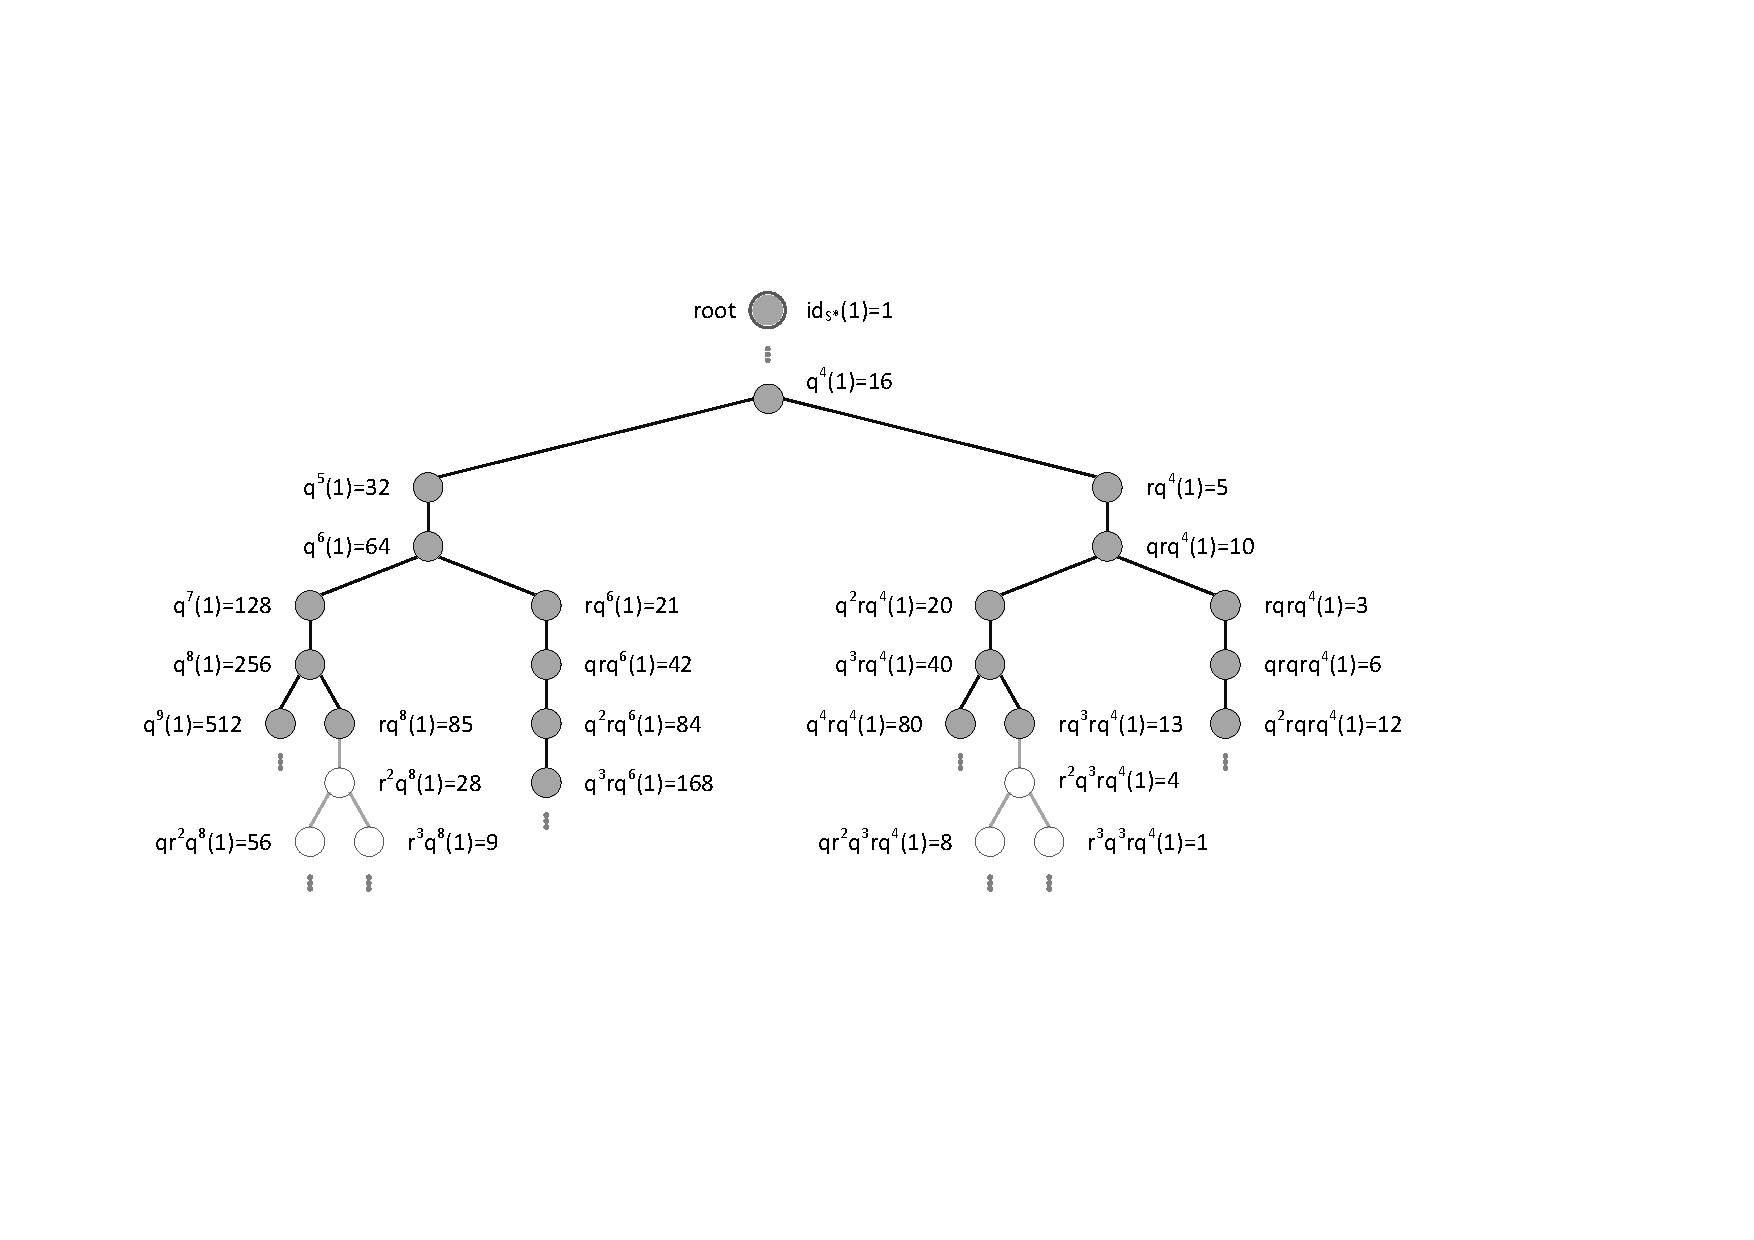
\includegraphics[trim=2.3cm 5.8cm 5.9cm 4.8cm, 
	width=1.00\textwidth,page=1]{figures/caytree.pdf}
	\caption{Small section of $H_T$ with darkly highlighted subtree $H_U$}
	\label{fig:1}
\end{figure}

\section{Defining the Tree}
The starting point for specifying our tree is $H_U$. Due to its
significance, we first concertize $H_U$ by the definition~\ref{def:H_U}
below, which establishes four essential characteristics.

\pagebreak
\begin{definition}
The graph $H_U$ possess the following key properties:
\begin{itemize}
	\item \mbox{\boldmath$H_U$} \textbf{is a directed graph (digraph):} Fundamentally, when we consider the more general case, an undirected graph as a triple $(V,E,\psi)$, the incidence function maps an edge to an arbitary vertex pair $\psi : E\rightarrow\{X\subseteq V:\left|X\right|=2\}$. In a digraph, the set $V\times V$ represents ordered vertex pairs. Accordingly the incidence function is more specifically defined, namely as a mapping of the edges to that set $\psi : E\rightarrow\{(v,w)\in V\times V:v\neq w\}$, see \cite[p.~15]{Ref_Korte_Vygen}.
	\item \mbox{\boldmath$H_U$} \textbf{is a rooted tree:} According to Rosen \cite[p.~747]{Ref_Rosen}, a rooted tree is "a tree in which one vertex has been designated as the root and every edge is directed away from the root." Peculiarly, this definition considers the directionality as an inherent part of rooted trees. Unlike Mehlhorn and Sanders \cite[p.~52]{Ref_Mehlhorn_Sanders}, for example, who distinguish between an undirected and directed rooted tree.
	\par\smallskip
	\textit{Note: As long as we do not stipulate that vertices may collapse, it is absolutely guaranteed that the graph is a tree.}
	\item \mbox{\boldmath$H_U$} \textbf{is an out-tree:} There is exactly one	path from the root to every other node \cite[p.~52]{Ref_Mehlhorn_Sanders}, which means that edge directions go from parents to children \cite[p.~108]{Ref_Du_Ko_Hu}. This property is implied in Rosen's definition for a rooted tree as well by saying "every edge is directed away from the root." An out-tree is sometimes designated as \textit{out-arborescence} \cite[p.~108]{Ref_Du_Ko_Hu}.
	\item \mbox{\boldmath$H_U$} \textbf{is a labeled tree:} For defining a labeled graph, Ehrig et al. \cite[p.~23]{Ref_Ehrig_etal} use a label alphabet consisting of a vertex label set and an edge label set. Since we only label the vertices, in our case the specification of a vertex label set $L_V$ together with the vertex label function $l_V:V\rightarrow L_V$ is sufficient. Originally, we said vertex labels are strings over the alphabet $S=\{q,r\}$, through which the free monoid $S^*$ is generated. We illustrate labeling $H_U$ by defining $l_{V(H_U)}(v)=ev^0_{S^*}(l_{V(G)}(\iota(v)),1)$, whereby $\iota:V(H_U)\hookrightarrow V(G)$ is the inclusion map \cite[p.~142]{Ref_Childs} from the set of vertices of $H_U$ to the set of vertices from the previously defined Cayley graph $G$.
\end{itemize}
\label{def:H_U}
\end{definition}

\par\medskip
We define a tree $H_C$ by taking the tree $H_U$ as a basis and for every
vertex $v\in V(H_U)$ satisfying $2\mid l_{V(H_U)}(v)$, we contract the
incoming edge. We attach the label of the parent of $v$ to the new
vertex, which results by replacing (merging) the two overlapping
vertices that the contracted edge used to connect. Visually, we
obtain $H_C$ by contracting all edges in $H_U$ that have an even-labeled 
target vertex, which (due to contraction) gets "merged into its parent." 
Edge contraction is occasionally referred to as \textit{collapsing an 
edge}. For more details and examples on edge contraction, one can see
Voloshin \cite[p.~27]{Ref_Voloshin} and Loehr \cite{Ref_Loehr}.

\par\medskip
The tree $H_C$ is a \textit{minor of $H_U$}, since it can be obtained
from $H_U$ "by a sequence of any vertex deletions, edge deletions and
edge contractions" \cite[p.~32]{Ref_Voloshin}. The sequence of contracting
the edges between adjacent (in our case even-labeled) vertices is called
\textit{path contraction}.

\par\medskip
A small section of the tree $H_C$ is shown in figure~\ref{fig:2}. Other
definitions of the same tree exist, see for example Conrow 
\cite{Ref_Conrow} or Bauer \cite[p.~379]{Ref_Bauer}.

\begin{figure}
	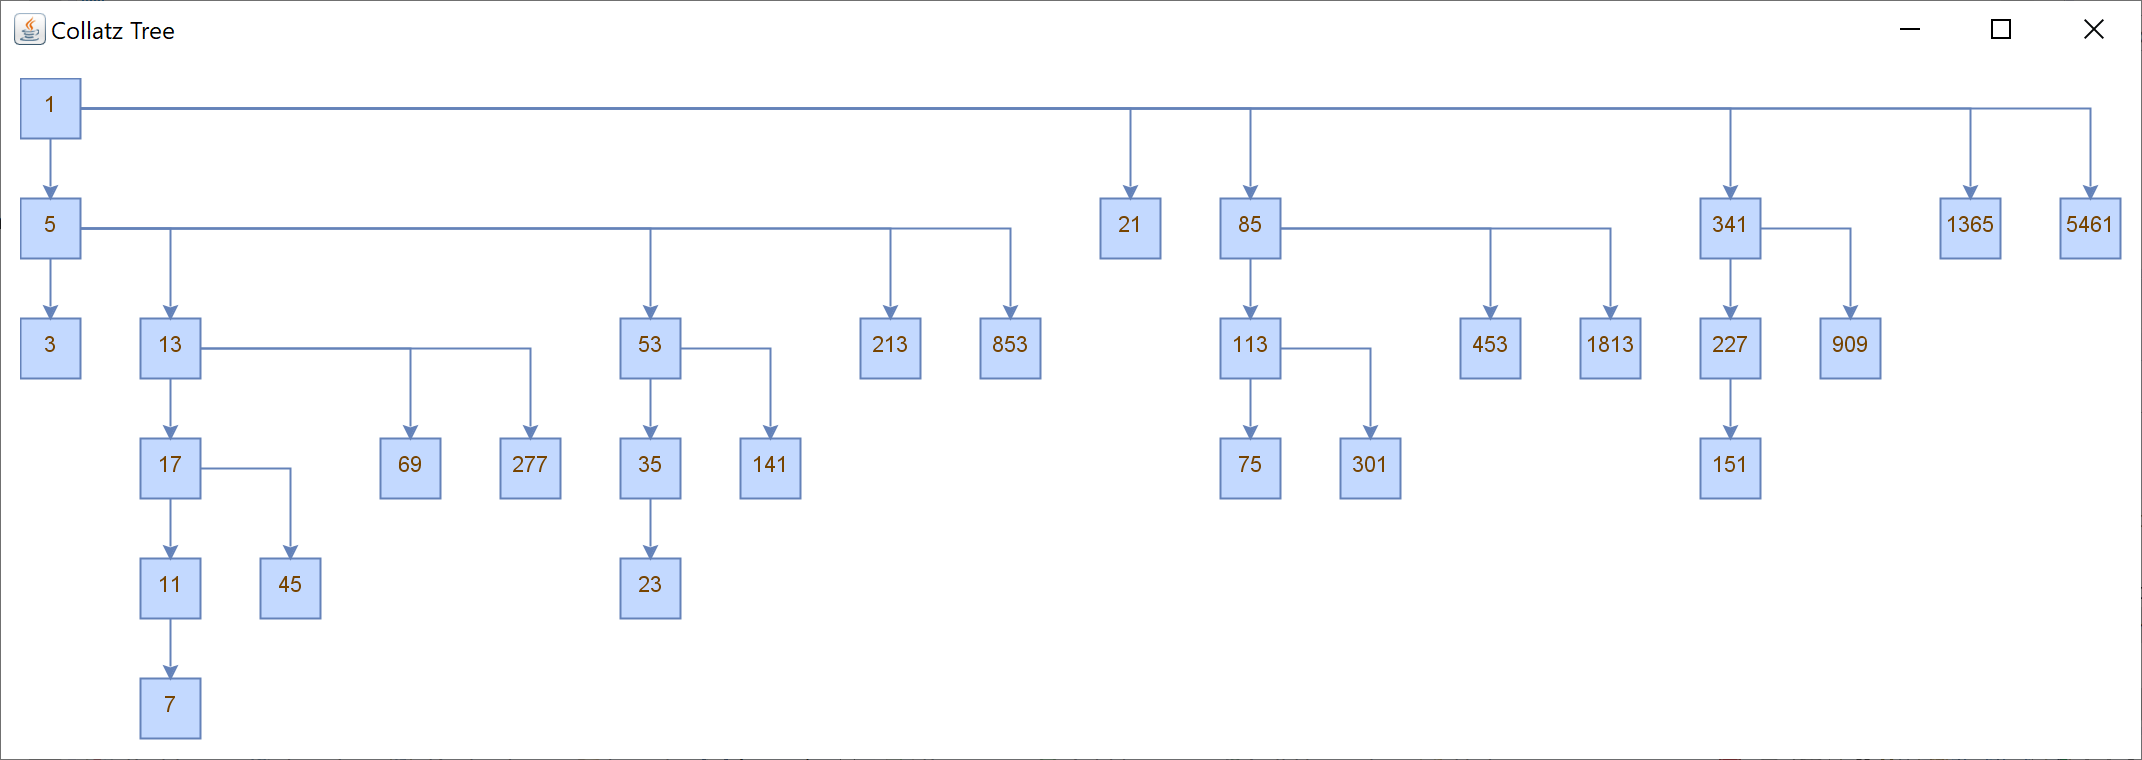
\includegraphics[width=1.00\textwidth]{figures/h_c.png}
	\caption{Small section of $H_C$ (displaying the trivial cycle is waived)}
	\label{fig:2}
\end{figure}

\section{Relationship of successive nodes in \mbox{$H_C$}}

Let $v_1$ and $v_{n+1}$ be two vertices of $H_C$, where $v_1$ is reachable from $v_{n+1}$ with $level(v_1)-level(v_{n+1})=n$. Hence, a path $(v_{n+1},\ldots,v_1)$ exists between these two vertices. Theorem~\ref{theo:1} specifies the following relationship between $v_1$ and $v_{n+1}$.

\par\medskip
\begin{theorem}
	\label{theo:1}
	$l_{V(H_C)}(v_{n+1})=3^nl_{V(H_C)}(v_1)\prod_{i=1}^{n}\left(1+\frac{1}{3l_{V(H_C)}(v_{i})}\right)2^{-\alpha_i}$.
	In order to simplify readability, we waive writing down the vertex label function and put it shortly:\\
	$v_{n+1}=3^nv_1\prod_{i=1}^{n}\left(1+\frac{1}{3v_{i}}\right)2^{-\alpha_i}$.
	The value $\alpha_i\in\mathbb{N}$ is the number of edges which have been contracted between $v_i$ and $v_{i+1}$ in $H_U$.
\end{theorem}

In order to demonstrate the construction produced by theorem~\ref{theo:1} in an illustrative fashion, example~\ref{ex:vertices} runs through a concrete path in $H_C$.

\par\medskip
\begin{example}
	\label{ex:vertices}
	For example, the two vertices $v_1=45$ and $v_{1+3}=v_4=5$ are 
	connected
	via the path $(5,13,17,45)$, see figure~\ref{fig:2}. Furthermore, one
	can retrace in figure~\ref{fig:3} the uncontracted path between these
	two nodes within $H_U$. When applied to this example,
	theorem~\ref{theo:1} produces the following:	
	\begin{center}
		$5=v_{1+3}=3^3*45*\left(1+\frac{1}{3*45}\right)*2^{-3}
		*\left(1+\frac{1}{3*17}\right)*2^{-2}
		*\left(1+\frac{1}{3*13}\right)*2^{-3}$
	\end{center} 
\end{example}
\begin{proof}
	\label{proof:1}
	This relationship of successive nodes can simply be proven inductively. For the base case, we set $n=1$ and retrieve
	\begin{center}
		$v_{1+1}=3v_1\left(1+\frac{1}{3v_1}\right)2^{-\alpha_1}
		=\left(3v_1+1\right)2^{-\alpha_1}=v_2$
	\end{center}
	The path from $v_2$ to $v_1$ can conformly be expressed by a string $rq\cdots q$ of $S^*$, because of $v_1=r\circ q^{\alpha_1}\left(v_2\right)$. We set $n=n+1$ for the step case, which leads to
	\begin{equation*}
	\begin{array}{cl}
	v_{n+2} &
	=3^{n+1}v_1\prod_{i=1}^{n+1}\left(1+\frac{1}{3v_i}\right)2^{-\alpha_i}\\
	&
	=3^{n+1}v_1\left(1+\frac{1}{3v_{n+1}}\right)2^{-\alpha_{n+1}}\prod_{i=1}^{n}\left(1+\frac{1}{3v_i}\right)2^{-\alpha_i}\\
	&
	=3\left(1+\frac{1}{3v_{n+1}}\right)2^{-\alpha_{n+1}}3^nv_1\prod_{i=1}^{n}\left(1+\frac{1}{3v_i}\right)2^{-\alpha_i}\\
	&
	=3\left(1+\frac{1}{3v_{n+1}}\right)2^{-\alpha_{n+1}}v_{n+1}\\
	&
	=\left(3v_{n+1}+1\right)2^{-\alpha_{n+1}}
	\end{array}
	\end{equation*}
	In this case the path from $v_{n+2}$ to $v_{n+1}$ is conformly 
	expressable by a string $rq\cdots q$ of $S^*$ too, since
	$v_{n+1}=r\circ q^{\alpha_{n+1}}\left(v_{n+2}\right)$.
\end{proof}

Even though the tree may theoretically contain two or more identically labeled vertices, it is essential to emphasize that we only consider such paths $(v_{n+1},\ldots,v_1)$ whose vertices are all labeled differently. Later in section~\ref{sec:cycles}, we even require that identically labeled nodes are one and the same. In order to correctly determine successive nodes using theorem~\ref{theo:1}, we must consider the halting conditions. These are specified in Definition~\ref{def:halting_condition}.

\begin{definition}
	\label{def:halting_condition}
	When determining successive nodes starting at $v_1$ according to theorem~\ref{theo:1}, we halt if one of the following two conditions is fulfilled:
	\begin{enumerate}
		\item $v_{n+1}=1$
		\item $v_{n+1}\in\{v_1,v_2,\ldots,v_n\}$
	\end{enumerate}
	If the first condition applies, the Collatz conjecture is true for a specific sequence. When the second condition is fulfilled, the sequence has led to a cycle. For every starting node, except the root node (labeled with $1$), the Collatz conjecture is consequently falsified. Let us consider the example $v_1=13$, where the algorithm halts after two iterations, because the first condition is met:
	\[
	v_{n+1}=3^2\cdot\left(1+\frac{1}{3\cdot13}\right)\left(1+\frac{1}{3\cdot5}\right)\cdot2^{-7}=1
	\]
	
	If we examine the case $v_{1}=1$, we realize that the algorithm finishes after the first iteration, since both halting conditions are true. The sequence stops because the final node labeled with $1$ is reached. Furthermore, the sequence has led to a cycle:
	\[
	v_{n+1}=3\cdot\left(1+\frac{1}{3}\right)2^{-2}=1
	\]
	
	The trivial cycle is the only sequence where both conditions are fulfilled.
\end{definition}

\noindent
Theorem~\ref{theo:1} can be used for specifying the condition of a cycle as follows:

\begin{equation}
\label{eq:func_cycle}
\begin{array}{l}
v_{1}=3^nv_1\prod_{i=1}^{n}\left(1+\frac{1}{3v_i}\right)2^{-\alpha_i}
\\[\medskipamount]
2^{\alpha_1+\cdots+\alpha_n}=\prod_{i=1}^{n}\left(3+\frac{1}{v_i}\right)
\end{array}
\end{equation}

A similar condition has been formulated by Hercher \cite{Ref_Hercher} and Eric Roosendaal \cite{Ref_Roosendaal_2020}. Taking a first look at equation~\ref{eq:func_cycle}, we are able to recognize the trivial cycle for $n=1$. One might easily come to the false conclusion that the term only results in a natural number for this trivial cylce, since we are multiplying fractions. The following counterexample, starting at $v_1=31$, disproves this assumption:
\begin{equation*}
20480=\left(3+\frac{1}{31}\right)\left(3+\frac{1}{47}\right)
\left(3+\frac{1}{71}\right)\left(3+\frac{1}{107}\right)\left(3+\frac{1}{161}\right)\left(3+\frac{1}{121}\right)\left(3+\frac{1}{91}\right)\left(3+\frac{1}{137}\right)\left(3+\frac{1}{103}\right)
\end{equation*}

According to OESIS \cite{Ref_OESIS}, the integer $v_1=31$ is called \textit{self-contained}. The term self-contained is based on the fact that the node $v_{n+1}=v_{10}=155$ is divisible by the starting node $v_1=31$. Moreover, $v_{10}$ results from applying one and the same function (in this case the Collatz function) using $v_1$ as input, see also Guy \cite[p.~332]{Ref_Guy}. For such a case equation~\ref{eq:func_cycle} leads to a natural number, but not necessarily to a cycle. A cycle only occurs if the term results in a power of two. One example is the trivial cycle. We find another case when we choose the factor $5$ instead of $3$:
\begin{center}
	$128=2^7=\left(5+\frac{1}{13}\right)\left(5+\frac{1}{33}\right)
	\left(5+\frac{1}{83}\right)$
\end{center}

The above example shows that non-trivial cycles can be found if we generalize the Collatz conjecture by replacing the factor $3$ with the variable $k$. We study this generalized form and the occurance of cycles in section~\ref{sec:cycles}. A detailed elaboration of the divisibility and a deeper understanding of the tree $H_C$ needs to be performed in order to get towards any proof of the Collatz conjecture.

%\par\medskip\noindent
%Generally, for any variant $kx+1$ it applies that if $v_1\mid v_{n+1}$, the the product is natural:
%\begin{equation*}
%	\prod_{i=1}^n\left(k+\frac{1}{v_i}\right)\in \mathbb{N}
%\end{equation*}

\begin{figure}
	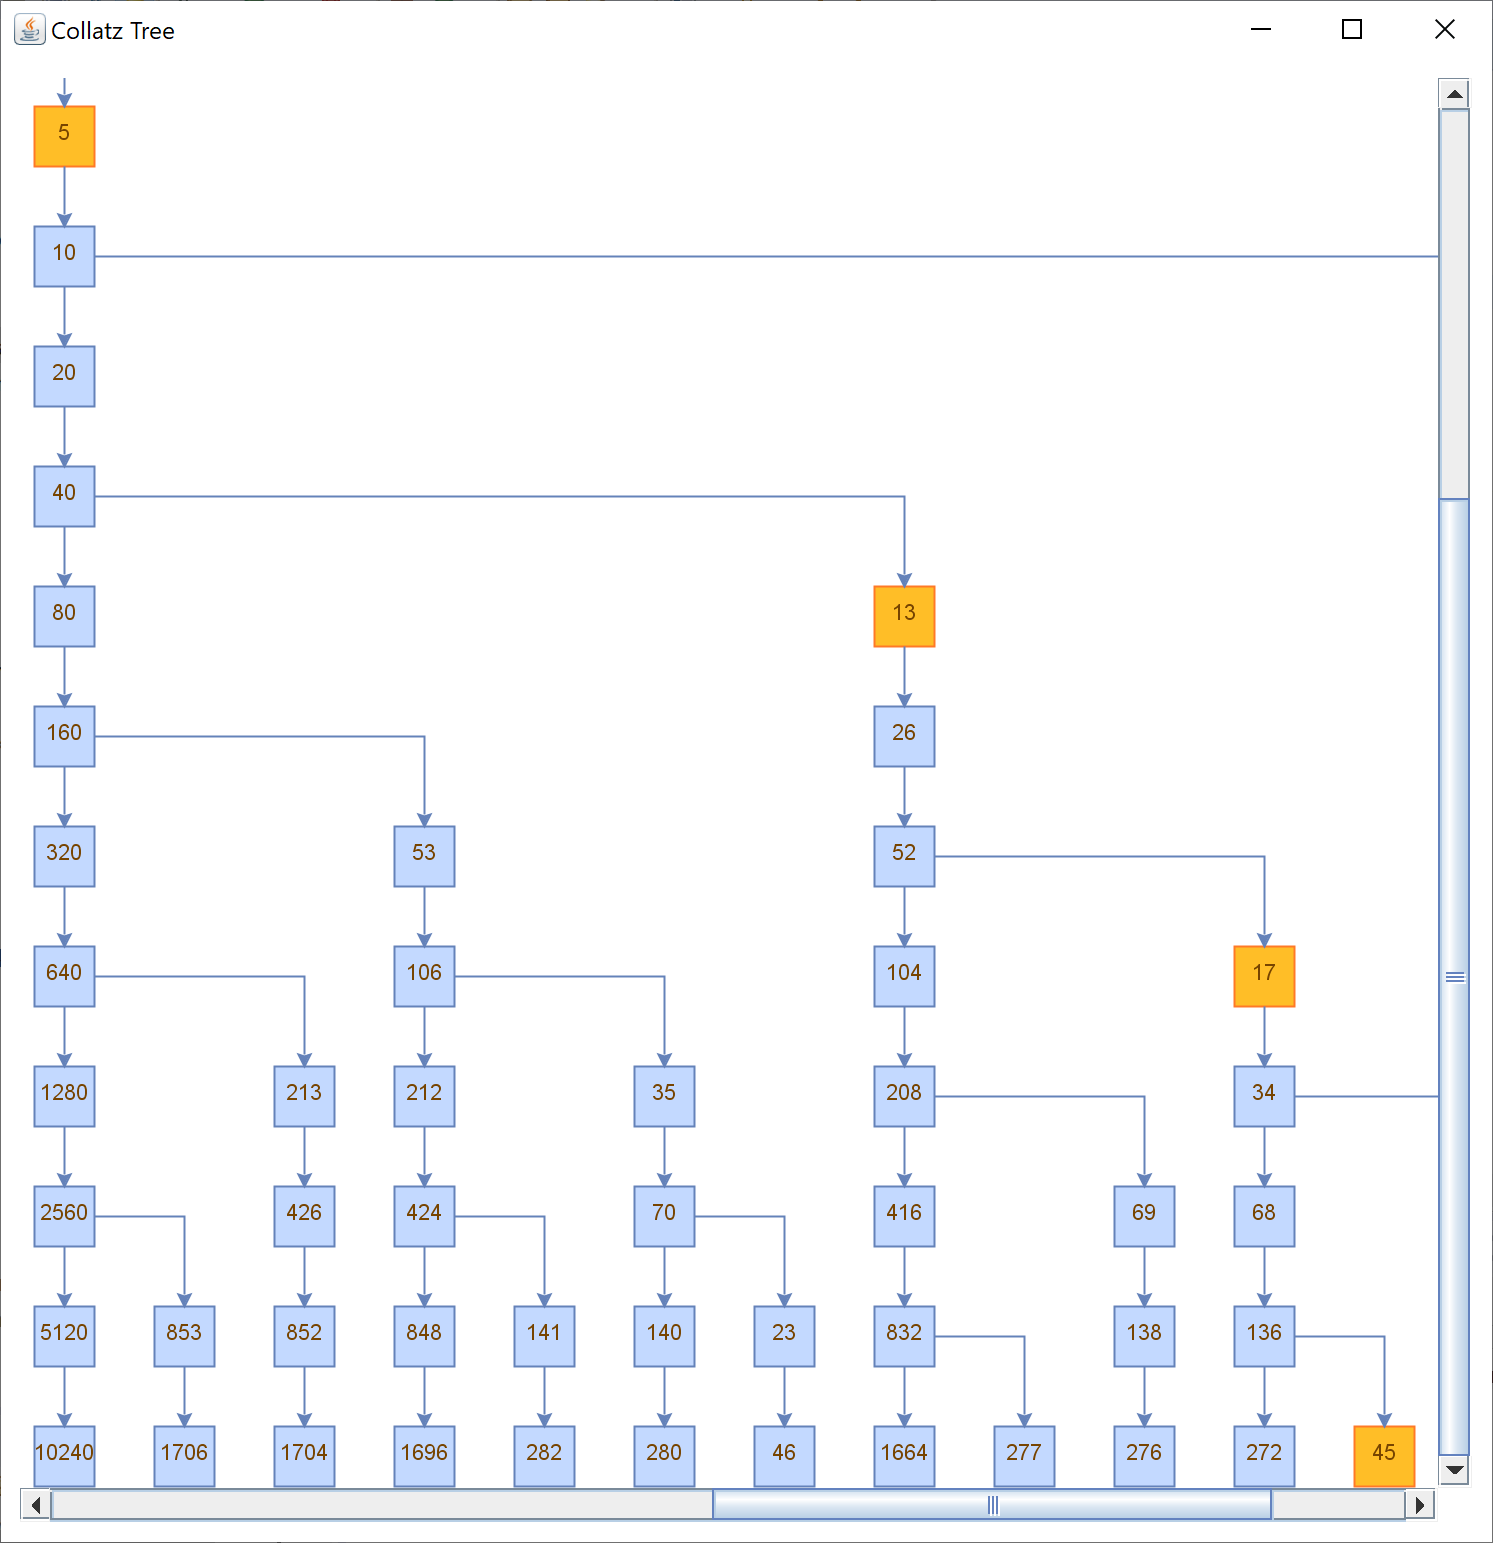
\includegraphics[width=1.00\textwidth]{figures/h_u.png}
	\caption{Section of $H_U$ containing the path from $5$ to $45$}
	\label{fig:3}
\end{figure}

\section{Relationship of sibling nodes in \mbox{$H_C$}}
In a rooted tree, vertices which have the same parent are called "siblings" \cite[p.~702]{Ref_Johnsonbaugh}, \cite[p.~747]{Ref_Rosen}. Sibling vertices accordingly have the same level.

\par\medskip
Let $w$ be a vertex, from which a path exists to the vertex $v_1$. Let $v_2$ be the immediate right-sibling of $v_1$, then $l_{V\left(H_C\right)}\left(v_2\right)=4*l_{V\left(H_C\right)}\left(v_1\right)+1$. This fact has been expressed differently by Kak \cite{Ref_Kak_2014} as follows: "If an odd number $a$ leads to another odd number (after several applications of the Collatz transformation) $b$, then $4a+1$ also leads to $b$."

\par\medskip
Applied to our approach, consider $w$ as the parent of $v_1$ and $v_2$. Suppose, in $H_U$, a path consisting of $n+1$ edges goes from $w$ to $v_1$. Then we can straightforwardly show that $n$ edges in $H_U$ have been contracted between both nodes $w$ and $v_1$ and $n+2$ edges between $w$ and $v_2$ (for simplicity we again omit writing the label function):
\begin{equation*}
\begin{array}{l}
		v_1=\frac{w*2^n-1}{3}
		\\[\medskipamount]
		v_2=\frac{w*2^{n+2}-1}{3}=4*v_1+1
\end{array}
\end{equation*}

For example, $n=3$ edges in $H_U$ have been contracted between $w=5$ and $v_1=13$ and $n+2=5$ edges between $w$ and $v_2=53$, whereby in $H_C$, the vertex $v_2$ is the right-sibling of $v_1$ and these two sibling vertices are immediate children of $w$.

\section{A vertex's \mbox{$n$}-fold left-child and right-sibling in \mbox{$H_C$}}
Referring to the "left-child, right-sibling representation" of rooted trees \cite[p.~246]{Ref_Cormen_Leiserson_Rivest_Stein}, the function $\textit{left-child}:V\rightarrow V$ returns the leftmost child of a vertex $v$. Nesting this function $n$ times leads to the definition of a vertex's $n$-fold left-child, which is given by $\textit{left-child}^n(v)$. As shown in figure~\ref{fig:2}, for example $\textit{left-child}^3(13)=7$.

\par\medskip
The function $\textit{right-sibling}:V\rightarrow V$ points to the sibling of a vertex $v$ immediately to its right \cite[p.~246]{Ref_Cormen_Leiserson_Rivest_Stein}. If this function is nested $n$ times, we get a vertex's $n$-fold right-sibling defined by $\textit{right-sibling}^n(v)$. One example is $\textit{right-sibling}^2(113)=1813$ which has been demonstrated in figure~\ref{fig:2} too.

\par\medskip
Let $w$ be a vertex in $H_C$ and $v_0$ the left-child of $w$. The $n$-fold right-sibling of $v_0$ can be calculated as follows:
\begin{equation}
\label{eq:nfold_right_sibling}
	v_n=\textit{right-sibling}^n(v_0)=\frac{1}{3}*\left(w*2^{2*n+\pi_3(w\bmod 3)}-1\right)
\end{equation}

The function $\pi_3$ is the self-inverse permutation (involution):
\begin{equation}
\label{eq:pi_3}
	\pi_3=\left(\begin{array}{cc}
	1 & 2\\
	2 & 1
	\end{array}\right)
\end{equation}
We consider permutations of the set $\{1,2\}$ and not of $\{0,1,2\}$, due to the fact that $w\bmod 3$ cannot be zero. A node $w$ in $H_C$, which is labeled by an integer divisible by $3$ is a leaf; and therefore such node has no left-child, more specifically it has no children at all.

\par\medskip
\noindent
When setting $n=0$, we trivially retrieve the vertex's $w$ left-child:
\begin{center}
	$v_0=\textit{left-child}(w)=\frac{1}{3}*\left(w*2^{\pi_3(w\bmod 3)}-1\right)$
\end{center}

\begin{example}
	\label{ex:siblings}
	Let us refer to figure~\ref{fig:2} again and pick out $w=5$. Then the
	vertex's $w$ left-child is $v_0=3$ and the threefold right-sibling
	$v_3=213$:

	\begin{equation*}
	\begin{array}{l}
		v_0=\frac{1}{3}*\left(5*2^{\pi_3(5\bmod 3)}-1\right)=3
		\\[\medskipamount]
		v_3=\frac{1}{3}*\left(5*2^{2*3+\pi_3(5\bmod 3)}-1\right)=213
	\end{array}
	\end{equation*}
\end{example}

\section{Left-child and right-sibling in the \mbox{$5x+1$} variant of \mbox{$H_C$}}
In the following we take a look at the $5x+1$ variant of $H_C$. We name this graph $H_{C,5}$ and must note that it is not a tree and moreover that not all of its vertices are reachable from the root. We define the permutation $\pi_5$ as follows:
\begin{center}
	$\pi_5=\left(\begin{array}{cccc}
		1 & 2 & 3 & 4\\
		4 & 3 & 1 & 2
	\end{array}\right)$	
\end{center}

Next, by letting $w$ be a vertex in $H_{C,5}$ and $v_0$ the left-child of $w$
we obtain the $n$-fold right-sibling of $v_0$ by the function that
is slightly different to the one defined by \ref{eq:nfold_right_sibling}:
\begin{equation}
\label{eq:nfold_right_sibling_5}
	v_n=\textit{right-sibling}^n(v_0)=\frac{1}{5}*\left(w*2^{4*n+\pi_5(w\bmod 5)}-1\right)
\end{equation}

Analogous to \ref{eq:pi_3} only permutations on the set without zero
\{1,2,3,4\} need to be considered, since $w\bmod 5$ cannot be zero.
Otherwise, if $w\equiv 0 (\bmod 5)$ which means that $w$ were labeled
by an integer divisible by 5, then the node $w$ has no successor in $H_{C,5}$.

\par\medskip
\noindent
By setting $n=0$, the function (above given by \ref{eq:nfold_right_sibling_5}) returns the left child of $w$:
\begin{center}
	$v_0=\textit{left-child}(w)=\frac{1}{5}*\left(w*2^{\pi_5(w\bmod 5)}-1\right)$
\end{center}

\begin{figure}
	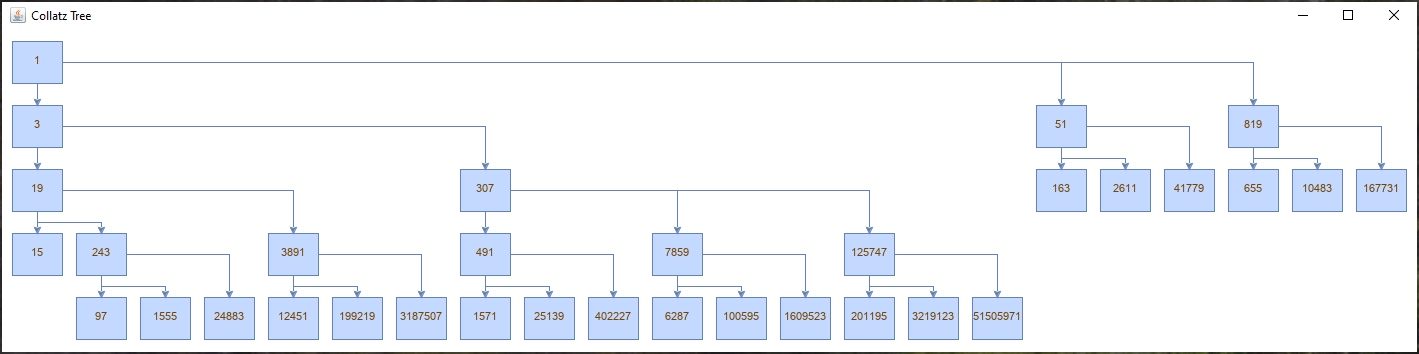
\includegraphics[width=1.00\textwidth]{figures/h_c5b.png}
	\caption{Section of the graph $H_{C,5}$ starting at its root (without branches that reflect a subsequence containing the trivial cycle)}
	\label{fig:4}
\end{figure}

Figure~\ref{fig:4} illustrates a small section of $H_{C,5}$ starting at its root. The particularly interesting thing about the graph $H_{C,5}$ is that it contains three cycles, the trivial cycle starting from the root $1,3$ and two non-trivial cycles $43,17,27$ and $83,33,13$. To be precise, three cycles are known (as it will become apparent later in section~\ref{sec:non_trivial_cycles}), and on the basis of present knowledge it cannot be ruled out with any certainty that other cycles exist.

\chapter{Binary Collatz Tree}
\label{ch:binary_tree}

\section{Some essentials on binary trees}
A binary tree is a rooted tree, where each node has at most two immediate successors. Those nodes, from which no edge goes out downward, are called leaves, the others are called internal nodes. In a full binary tree, all internal nodes have exactly two children \cite[p.~102]{Ref_Higham_2015}. Full binary trees have an odd number $2n+1$ of nodes. Of these $n+1$ are leaves and $n$ are inner nodes \cite[p.~134]{Ref_Kersting_Wakolbinger_2008}. Each node in a binary tree has a left subtree and a right subtree, which is why a binary tree is inherently recursive, since the left and right subtrees of the root are themselves binary trees \cite[p.~246-247]{Ref_Mazur_2010}. As it often pops up in combinatorial problems, the famous $n$-th Catalan number, named after the Belgian mathematician Eugène Catalan, comes in connection with binary trees into play. For $n\ge1$ it specifies the number of binary trees on $n$ vertices \cite[p.~247]{Ref_Mazur_2010}:
\[
B_n=\sum_{i=0}^{n-1}B_iB_{n-1-i}=\sum_{i=1}^{n}B_{i-1}B_{n-i}=\frac{1}{n+1}\binom{2n}{n}
\]

There is an interesting property that trees exhibit regarding abstract algebra. Let's have a look at the algebraic structure of magmas. Consider an element $x$ of a magma $(M,*)$ which is an iterated product of other elements in $M$. Such an element can be described by a planar (no edges cross each other) rooted binary tree whose $n$ leaves are labelled by these other elements $x_1,\ldots,x_n\in M$ \cite[p.~96]{Ref_Kalka_2016}.

Binary trees make well-suited data structures for storing information. With about $2^m$ data points (nodes), a search of a binary tree takes only about $m$ steps, compared to about $2^{m-1}$ steps which are required to search a simple list \cite[p.~84]{Ref_Benjamin_2009}.

\section{Transforming the Collatz tree into a binary tree}
Jan Kleinnijenhuis and Alissa M. Kleinnijenhuis \cite{Ref_Kleinnijenhuis_2020a} introduced a binary tree $T_{\ge0}$ by transforming the original Collatz tree $H_U$ into the Syracuse tree $H_{C,3}$, which in turn is transformed into the binary tree $T_{\ge0}$ as described next. The edges are changed according to the following procedure: whenever a parent node $w$ has edges to its child nodes $v_0,v_1,\ldots,v_n$, on the tree $H_{C,3}$, we draw an edge from $w$ to $v_0$, and edges from $v_i$ to $v_{i+1}$ for each $i=1,\ldots,n-1$, in the binary new tree. Note that the nodes $v_1,v_2,\ldots,v_n$ are sorted in increasing order of label $v_0<v_1<\ldots<v_n$, which is already given by \ref{eq:n_fold_right_sibling_k}. Figure~\ref{fig:bt3} and \ref{fig:bt3_rot} display that tree -- once in our standard layout and once reversed (from bottom to top).

\begin{figure}[H]
	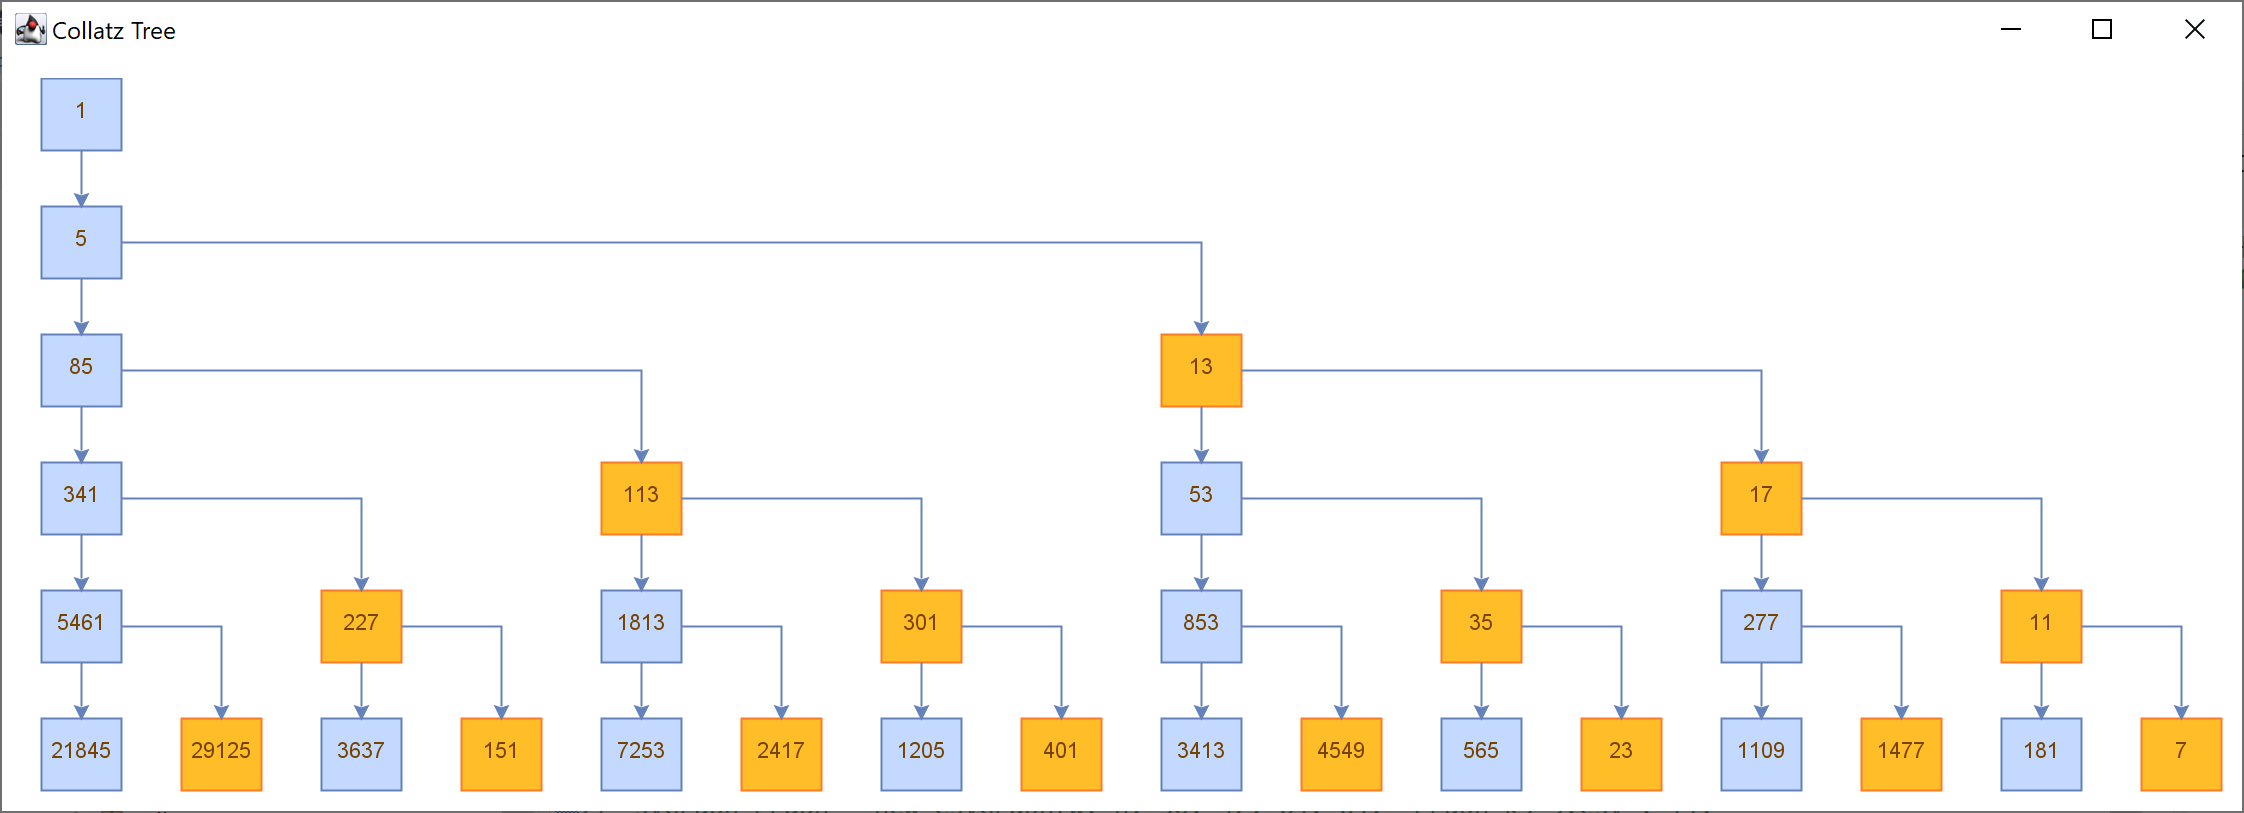
\includegraphics[width=1.00\textwidth]{figures/bt_3_t0.png}
	\caption{The Collatz Tree transformed to the binary tree $T_{\ge0}$}
	\label{fig:bt3}
\end{figure}

\vspace{-2em}
\begin{figure}[H]
	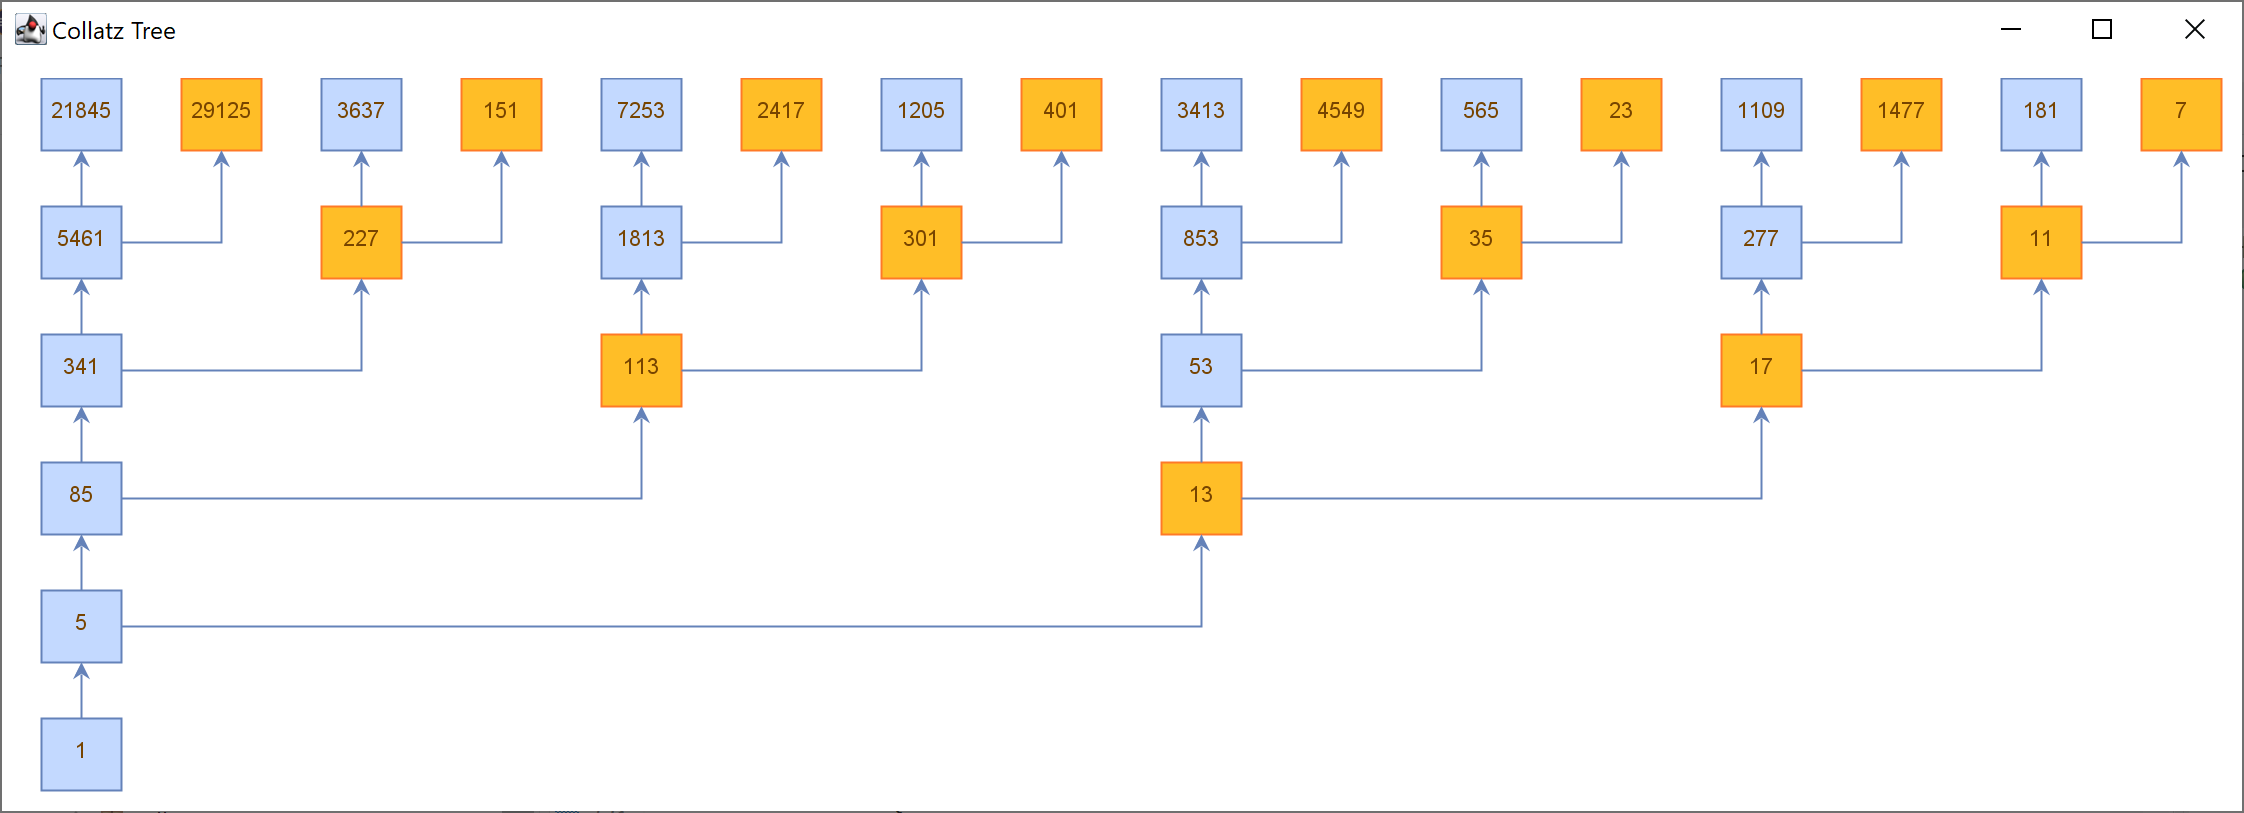
\includegraphics[width=1.00\textwidth]{figures/bt_3_t0_rot.png}
	\caption{The binary tree $T_{\ge0}$ with \textit{bottom-to-top} layout orientation}
	\label{fig:bt3_rot}
\end{figure}

\begin{remark}
	To clarify the terminology, it should be mentioned that Jan and Alissa M. Kleinnijenhuis in their manuscripts \cite{Ref_Kleinnijenhuis_2020a}, \cite{Ref_Kleinnijenhuis_2020b} denote the original Collatz tree $T_C$ while we call it $H_U$. They denote the Syracuse Tree $T_T$ which in our nomenclature is referred to as $H_{C,3}$.
\end{remark}

Nodes that are highlighted orange in figures~\ref{fig:bt3},~\ref{fig:bt3_rot} are called \textit{prunable} and they are exactly those nodes resulting as output of the \textit{Rightward} function. For navigating within this binary tree, Jan Kleinnijenhuis and Alissa M. Kleinnijenhuis \cite{Ref_Kleinnijenhuis_2020a} defined an \textit{Upward} function $U(n)$ and a \textit{Rightward} function $R(n)$ as follows:

\begin{equation}
\label{eq:bintree_3_rightward_upward}
\setlength{\arraycolsep}{1.6em}
\begin{array}{cc}
U(n)=\begin{cases}
        4n+1	&	n\equiv 1\pmod 6\\
        16n+5	&	n\equiv 5\pmod 6
    \end{cases} &
R(n)=\begin{cases}
    \nicefrac{(2^2n-1)}{3}	&	n\equiv 1\pmod{18}\\
    \nicefrac{(2^3n-1)}{3}	&	n\equiv 5\pmod{18}\\
    \nicefrac{(2^4n-1)}{3}	&	n\equiv 7\pmod{18}\\
    \nicefrac{(2^1n-1)}{3}	&	n\equiv 11\pmod{18}\\
    \nicefrac{(2^2n-1)}{3}	&	n\equiv 13\pmod{18}\\
    \nicefrac{(2^1n-1)}{3}	&	n\equiv 17\pmod{18}
\end{cases}
\end{array}
\end{equation}

The domain and codomain of both functions consist of the two residue classes $[1]_6,[5]_6$, which form the multiplicative (cyclic) group $\mathbb{Z}^\ast_6=\{1,5\}=<5>$. Consequently, the domain and codomain exclude all integers divisible by $2$ and $3$, which is due to the fact that this binary tree (just like our tree $H_{C,3}$) does not contain even numbers and additionally all leaves -- namely those nodes labeled with an integer divisible by three -- were deleted. The function $U(n)$ is very similar to the function~\ref{eq:next_sibling_k3} and to the more general function~\ref{eq:n_fold_right_sibling_k} (when setting $n=1,k=3$) which both calculate the right-sibling of a given vertex. This is clear, since siblings (parallel) in $H_{C,3}$ are successors (serial) in the binary tree $T_{\ge0}$. In the end, for a node $v_0$ having a leaf as right-sibling in $H_{C,3}$, the function $U(v_0)$ is defined as $v_1=4v_0+1$ executed twice $v_1=4(4v_0+1)+1=16v_0+5$, because we must skip this leaf. Recall that all leafs in $H_{C,3}$ are excluded from the binary tree without exception. For any $n\in[5]_6$ it applies that $U(n)\equiv16n+5\equiv\boldsymbol{1}\bmod(6)$ since $6\mid16n+5-\boldsymbol{1}$ resulting in $6\mid16(5+k\cdot6)+5-\boldsymbol{1}$, see \ref{eq:congruence}, and analogously for any $n\in[1]_6$ it applies that $U(n)\equiv4n+1\equiv\boldsymbol{5}\bmod(6)$ since $6\mid4n+1-\boldsymbol{5}$ resulting in $6\mid4(1+k\cdot6)+1-\boldsymbol{5}$. Therefore executing the Upward function twice in a row leads unconditionally to $U^2(n)=16(4n+1)+5=4(16n+5)+1=64n+21$.

\begin{remark}
	While we displayed trees from top to down, it is sometimes usual to draw trees in a bottom-to-top fashion as Kleinnijenhuis \cite{Ref_Kleinnijenhuis_2020b} do. The Rightward function corresponds to what we call left-child and the Upward function relates to the right-child which is commonly used in the context of binary trees \cite[p. 246]{Ref_Mazur_2010}.
\end{remark}

Jan and Alissa M. Kleinnijenhuis \cite{Ref_Kleinnijenhuis_2020a} defined the set $N(T_C)=N(H_U)$ that contains the labels of all nodes, to which a path from the root in $H_U$ exists, in other words, this set contains all integers $n$ for which the orbit of $n$ under the (uncompressed) Collatz function~\ref{eq:func_collatz} converges to $1$. Furthermore they introduced $S_{\ge0}$ as the node set containing integers that are neither divisible by $2$ nor by $3$. The set $S_{-1}$ comprises on the contrary all numbers, which are divisible by $2$ or $3$. In order to comprehend the structure of these sets $S$, let us take a look at the following list showing which tree includes which node set, see also the ancillary files of \cite{Ref_Kleinnijenhuis_2020a}, \cite{Ref_Kleinnijenhuis_2020b}:

\[\arraycolsep=0.6em\def\arraystretch{1.4}
\begin{array}{llll}
\text{Original Collatz tree} & N(T_C)=N(H_U)&=&\mathbb{N^+} \hspace{0.6em}\text{if the Collatz conjecture holds}\\
\text{Syracuse tree} & N(T_T)=N(H_{C,3})&=&N(T_C)\setminus2\mathbb{N}\\
\text{Binary tree}\hspace{0.6em}T_{\ge0}& N(T_{\ge0})=S_{\ge0}&=&N(T_C)\setminus S_{-1}\hspace{2.1em}=S_{0}\cup S_{1}\cup S_{2}\ldots\\
\text{Binary tree}\hspace{0.6em}T_{\ge1}& N(T_{\ge1})=S_{\ge1}&=&N(T_C)\setminus \bigcup_{i=-1}^{0}S_i=S_{1}\cup S_{2}\cup S_{3}\ldots\\
\text{Binary tree}\hspace{0.6em}T_{\ge j} & N(T_{\ge j})=S_{\ge j}&=&N(T_C)\setminus \bigcup_{i=-1}^{j-1}S_i=\bigcup_{i=j}^{\infty}S_i
\end{array}
\]

\par\medskip
Let us describe these sets using multiplicative groups. The set $S_{\ge0}=\mathbb{Z}^\ast_6$ can be understood as the multiplicative group modulo $6$ and the set $S_{-1}=\mathbb{Z}/6\mathbb{Z}\setminus\mathbb{Z}^\ast_6=\{0,2,3,4\}$ as the set of all non-invertible elements (non-units) of $\mathbb{Z}/6\mathbb{Z}$.

The set $S_0$ consists of all nodes resulting as output of $R(n)$ within the binary tree $T_{\ge0}$. These are the orange highlighted nodes displayed by figures~\ref{fig:bt3},~\ref{fig:bt3_rot}. In other words, $S_0$ is the codomain of the function $R(n)$ operating on nodes within $T_{\ge0}$. The binary tree $T_{\ge0}$ can be transformed to a (pruned) binary tree $T_{\ge1}$. For this, the prunable nodes will be deleted and their neighbors reconnected. The upward neighbor of a pruned node will then be identified as pruning candidate for a later transformation of the resulting tree $T_{\ge1}$ to a more pruned tree $T_{\ge2}$.

The set $S_1$ contains all nodes that are (as per the description above) identified as pruning candidates for the next transformation of $T_{\ge1}$ to $T_{\ge2}$. After having transformed $T_{\ge1}$ to $T_{\ge2}$, the more pruned binary tree $T_{\ge2}$ contains nodes that are identified as pruning candidates for another upcoming transformation of $T_{\ge2}$ to $T_{\ge3}$ -- these nodes are elements of the set $S_2$. This pruning algorithm is repeatedly applied in the same pattern. And in this way we obtain the sets $S_1,S_2,S_3,\ldots$ and so forth. Generally, we can write these sets in the form $S_j=\{n\in N(T_{j-1})\mid U^{-j}(n)\in S_0\}$. Kleinnijenhuis found out that the codomain $\mathbb{N}^U$ of the Upward function contains $5$ residue classes modulo $96$, namely $\{5, 29, 53, 77, 85\}=\mathbb{N}^U$ and the codomain $\mathbb{N}^R$ of the Rightward function comprises $27$ residue classes modulo $96$, namely $\{1, 7, 11, 13, 17, 19, 23, 25, 31, 35, 37, 41, 43, 47, 49, 55, 59, 61, 65, 67, 71, 73, 79, 83, 89, 91, 95\}=\mathbb{N}^R$. The union of both sets $\mathbb{N}^U\cup\mathbb{N}^R$ forms the non-cyclic multiplicative group $\mathbb{Z}^\ast_{96}=<\{5, 17, 31\}>$ (see \cite{Ref_Lang_2017}, \cite{Ref_OESIS_A033949}).

Let us take a closer look at the (cyclic) multiplicative group $\mathbb{Z}^\ast_{18}=\{1,5,7,11,13,17\}=<5>$ which has an order $ord(\mathbb{Z}^\ast_{18})=6$. Having the generator $5$ coprime to the modulus $18$, we obtain the congruence $5^{\phi(18)}\equiv1\pmod{18}$ in accordance with Euler's theorem \ref{eq:eulers_theorem}. This allows us to infer from $5^6\equiv5^{6(n+1)}\equiv5^j5^{6n+6-j}\equiv1\pmod{18}$ the congruences given by \ref{eq:homomorphism_congruences} (on the left).

If $m\mid n$, as in our case $3\mid18$, then the map $f:\mathbb{Z}^\ast_n\rightarrow \mathbb{Z}^\ast_m$ with $f(r\bmod n)=r\bmod m$ is a homomorphism as long as $\gcd(r\bmod n,n)=1$ leads to $\gcd(r\bmod m,m)=1$. By Euclid, we know that in the case $r$ is coprime to $n$ then it is also coprime to every factor $m$ of $n$. That is why a homomorphism exist to the congruences shown in \ref{eq:homomorphism_congruences} (on the right).

\begin{equation}
\label{eq:homomorphism_congruences}
\begin{array}{lllll}
	j=0 & [1]_{18}\cdot5^{6n+6}&\equiv1\pmod{18}&\hspace{4em}[1]_{18}\cdot4 &\equiv1\pmod{3}\\
	j=1 & [5]_{18}\cdot5^{6n+5}&\equiv1\pmod{18}&\hspace{4em}[5]_{18}\cdot8 &\equiv1\pmod{3}\\
	j=2 & [7]_{18}\cdot5^{6n+4}&\equiv1\pmod{18}&\hspace{4em}[7]_{18}\cdot16 &\equiv1\pmod{3}\\
	j=3 & [17]_{18}\cdot5^{6n+3}&\equiv1\pmod{18}&\hspace{4em}[17]_{18}\cdot2 &\equiv1\pmod{3}\\
	j=4 & [13]_{18}\cdot5^{6n+2}&\equiv1\pmod{18}&\hspace{4em}[13]_{18}\cdot4 &\equiv1\pmod{3}\\
	j=5 & [11]_{18}\cdot5^{6n+1}&\equiv1\pmod{18}&\hspace{4em}[11]_{18}\cdot2 &\equiv1\pmod{3}
\end{array}
\end{equation}

\newpage

Figure~\ref{fig:tree_transformations} shows the complete chain of tree transformations, beginning from the original Collatz tree, over the Syracuse tree to the binary tree and pruned ones.

% trim=left bottom right top
\begin{figure}[H]
	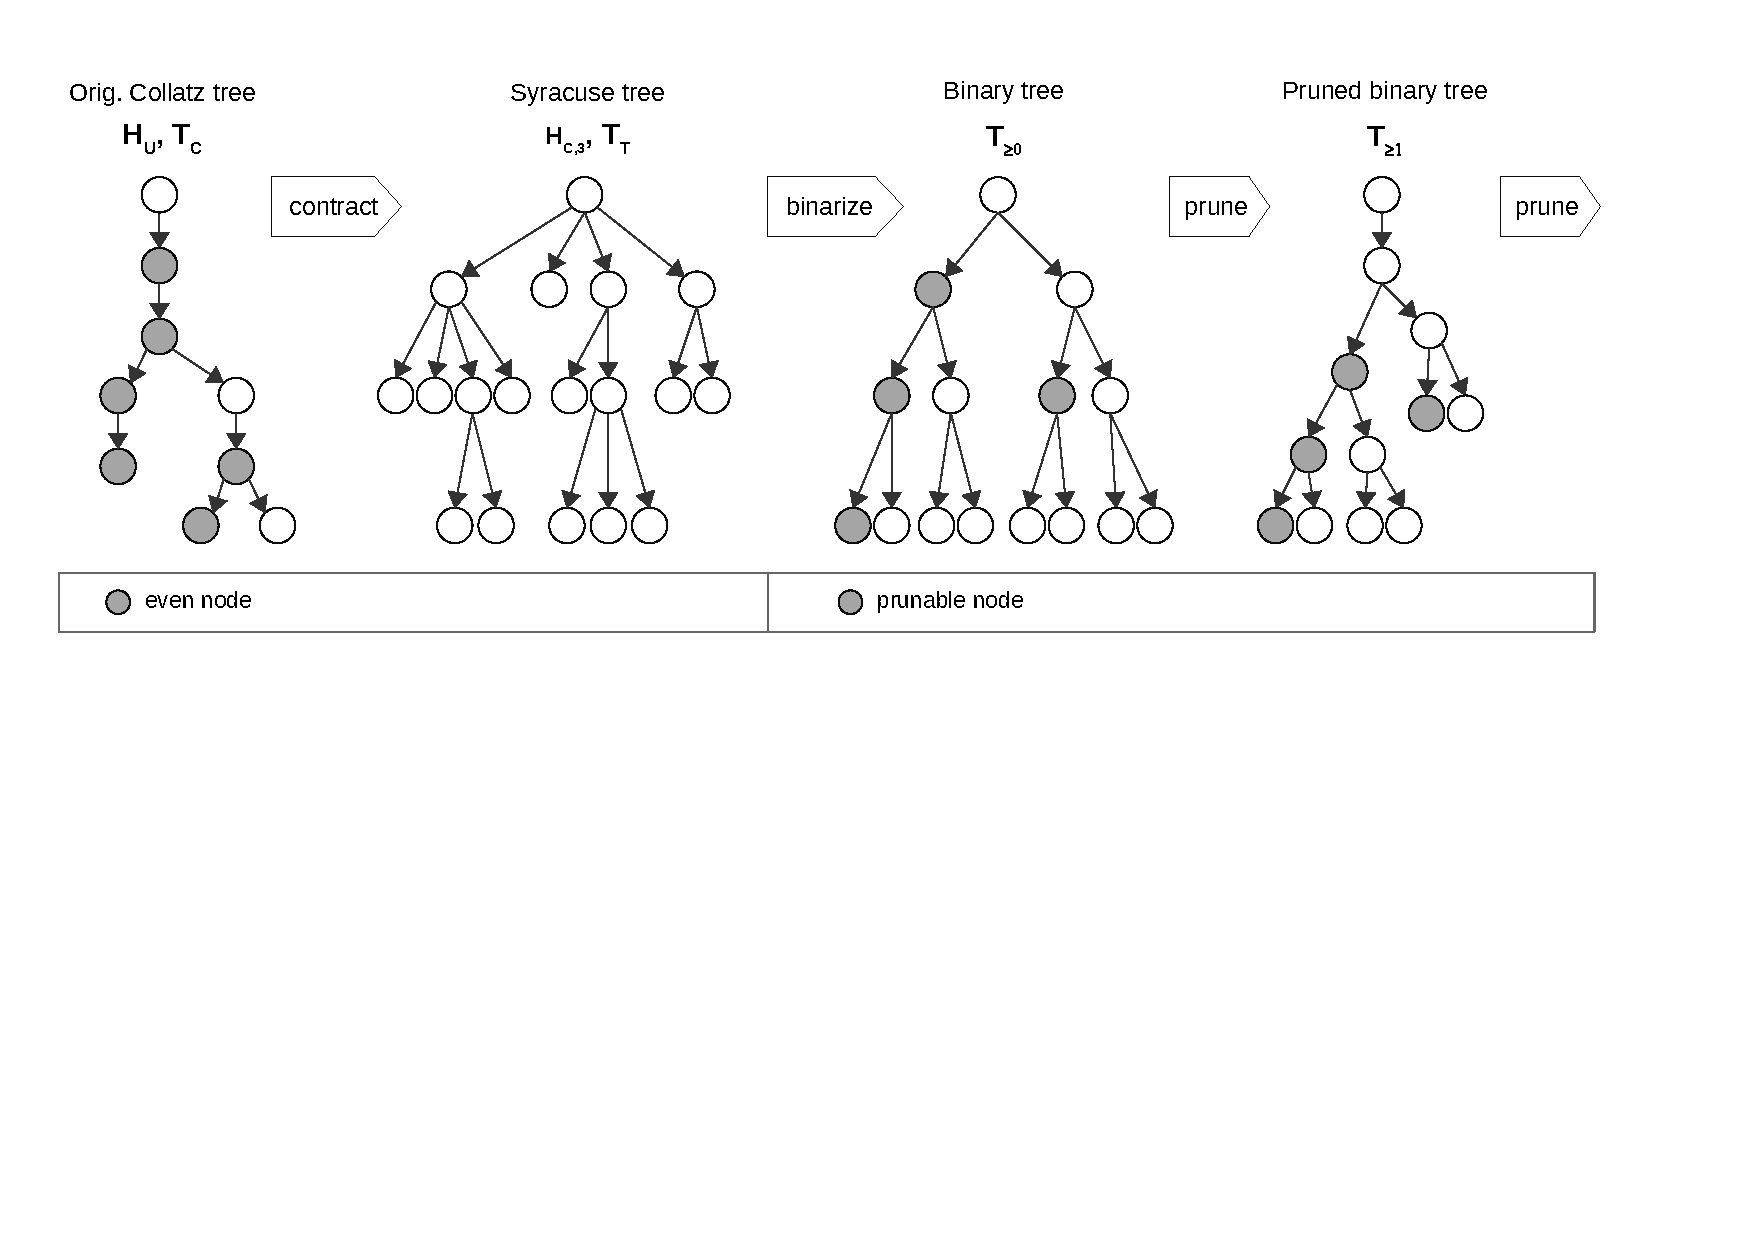
\includegraphics[trim=1.1cm 10cm 2.6cm 0.2cm, 
	width=1.00\textwidth,page=1]{figures/tree_transformations.pdf}
	\caption{Transformation chain, beginning from the original Collatz tree up to pruned binary trees}
	\label{fig:tree_transformations}
\end{figure}
\chapter{Cycles in the Collatz Tree}

\section{A remark about cycles}
\label{sec:cycles}
In graph theory, a path of length $n\geq 1$ that starts and ends at the same vertex is called a circuit. A circuit, in which no vertex is repeated with the sole exception that the initial vertex is the terminal vertex, is called a cycle. A cycle of length $n$ is referred to as an $n$-cycle. For these definitions, we rely on \cite[p.~599]{Ref_Rosen}, \cite[p.~35]{Ref_Benjamin_Chartrand_Zhang} and \cite[p.~445]{Ref_Chartrand_Zhang}. Furthermore, we call a cycle originating from the root a trivial cycle.

\begin{remark}
In order for the cycles to become graphically visible, we now require that in a graph $H$ two vertices $v_1$ and $v_2$ are one and the same if the label of both nodes are identical: $l_{V(H)}(v_1)=l_{V(H)}(v_2)\rightarrow v_1=v_2$. As a consequence, there is no guarantee that the graph precisely refers to the algebraic structure of a free monoid anymore. A free monoid requires that each of its elements can be written in one and only one way.
\end{remark}

When different nodes collapse on one, the graph is no longer necessarily a tree. Let us point to the monoid $S^\ast$, which we introduced in section \ref{sec:groups_graphs}. Take for example four of its elements, the empty string $e$, the strings $qqr$, $qqrqqr$, and $qqrqqrqqr$. These elements lie as well within the subset $U\subset T\subset S^\ast$, and they are represented by nodes of the tree $H_U$ that all have the same label $1=ev_{S^\ast}(qqr,1)=ev_{S^\ast}(qqrqqr,1)=ev_{S^\ast}(qqrqqrqqr,1)$. These nodes are one and the same, the root of $H_U$. Visually, then in $H_U$ a directed edge goes from the vertex labeled with $4$ back to the root node. Analogically, in $H_{C,3}$ a loop connects the root to itself, since due to the path contraction even labeled nodes do not exist in $H_{C,3}$. The  aforementioned example reflects the trivial cycle of the Collatz sequence.

Figure~\ref{fig:5} depicts a section of $H_{C,5}$, which includes the $3$-cycle $43,17,27$. Because of the two non-trivial cycles $43,17,27$ and $83,33,13$, in $H_{C,5}$ there does not exist a path between the root and the vertex $43$ and between the root and the vertex $83$. Hence, $H_{C,5}$ is said to be a disconnected graph. Generally, a graph is called a disconnected graph if it is impossible to walk (along its edges) from any vertex to any other \cite[pp.~46-47]{Ref_Benjamin_Chartrand_Zhang}.

\begin{figure}
	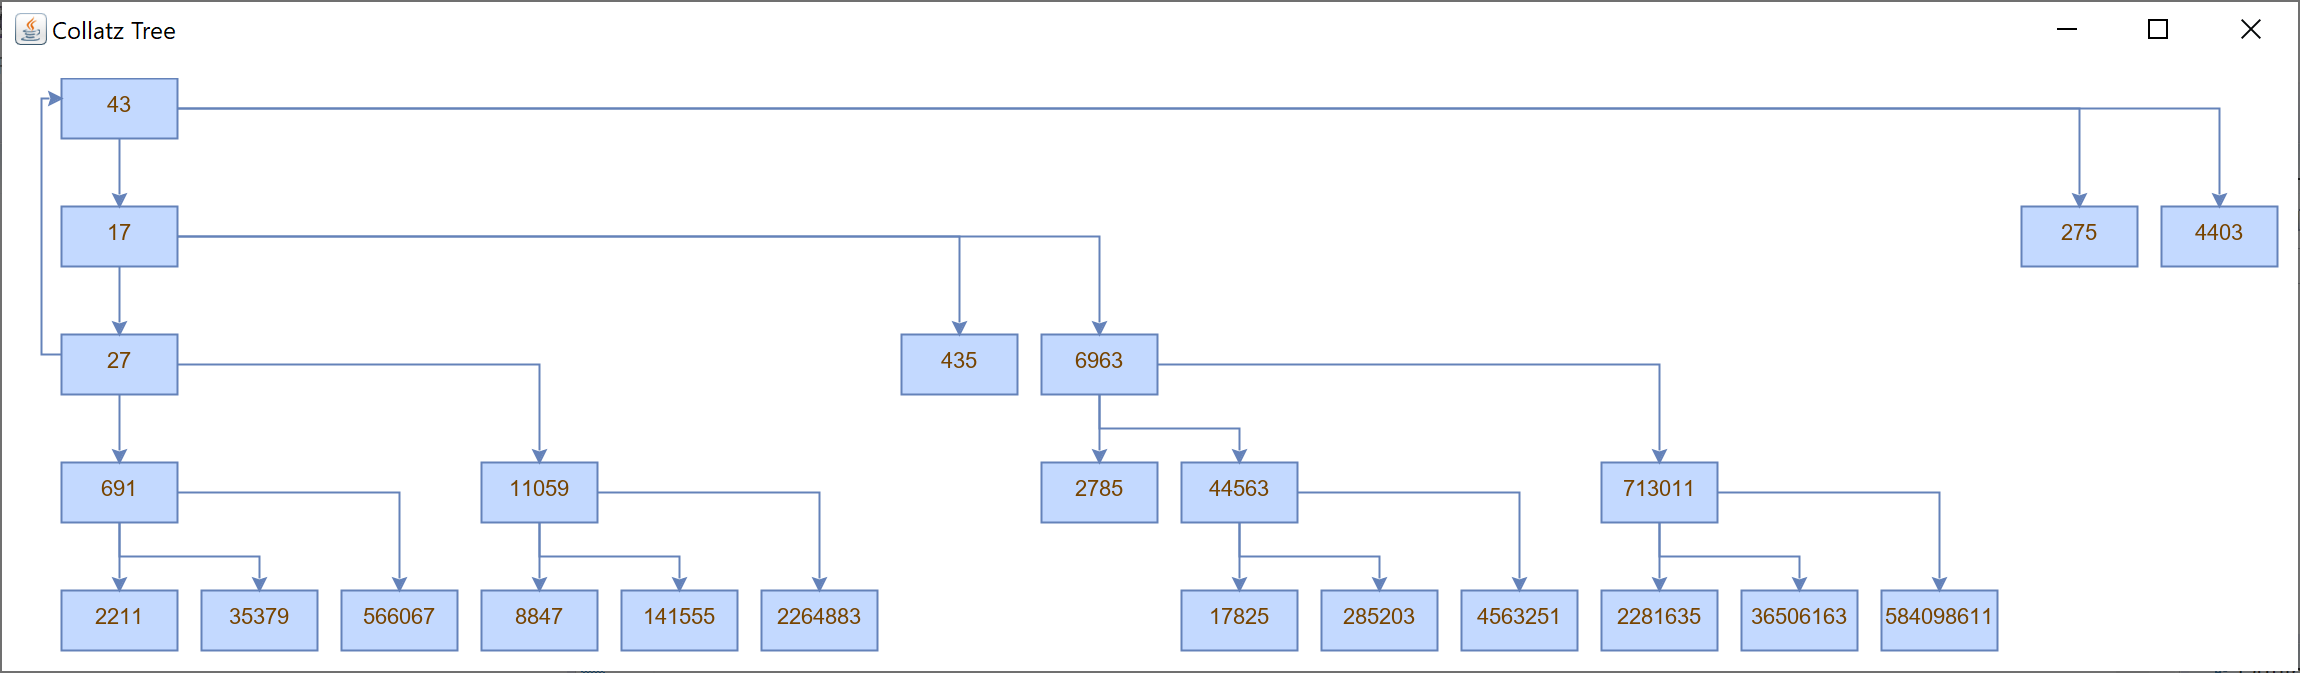
\includegraphics[width=1.00\textwidth]{figures/h_c5a.png}
	\caption{Section of $H_{C,5}$ including the $3$-cycle $43,17,27$}
	\label{fig:5}
\end{figure}

The following considerations focus on non-trivial cycles, and therefore on cycles that do not originate from the root, but cause the graph to be a disconnected graph. Utilizing the example of the graph $H_{C,5}$ we are able to deduct from the cycle $43,17,27$ the simple and self-evident equality $\textit{left-child}^3(43)=43$:
\begin{equation*}
\begin{array}{l}
\textit{left-child}(43)=\frac{1}{5}*\left(43*2^1-1\right)=17
\\[\medskipamount]
\textit{left-child}(17)=\frac{1}{5}*\left(17*2^3-1\right)=27
\\[\medskipamount]
\textit{left-child}(27)=\frac{1}{5}*\left(27*2^3-1\right)=43
\end{array}
\end{equation*}

Obviously, the authors note, it would be interesting to find out what circumstances enable a graph to have non-trivial cycles, whether it be the $5x+1$ variant, the $7x+1$ variant of $H_C$ or any variant $H_{C,k}$ with $k\geq 1$.

\section{\texorpdfstring{Which variants of $H_C$ have non-trivial cycles?}{Which variants of HC have non-trivial cycles?}}
\label{sec:non_trivial_cycles}
Let us refer to $H_{C,k}$. By having introduced and proven theorem~\ref{theo:1} we already started an assertion about the reachability of successive nodes in $H_{C,3}$. This reachability relationship can be generalized for any graph $H_{C,k}$ as follows:
\begin{equation}
\label{eq:generalized_reachability}
v_{n+1}=k^nv_1\prod_{i=1}^{n}\left(1+\frac{1}{kv_{i}}\right)2^{-\alpha_i}
\end{equation}

This generalization leads to the condition for an existence of an $n$-cycle in any $kx+1$ variant of $H_C$, which looks analogous to the condition given by equation~\ref{eq:func_cycle} that specifies $H_{C,3}$ has a cycle:
\begin{equation}
\label{eq:generalized_cycle}
2^\alpha=\prod_{i=1}^{n}\left(k+\frac{1}{v_i}\right)
\end{equation}

The natural number $\alpha$ is the sum of edges that have been contracted between the vertices $v_i$ forming the cycle, in other words $\alpha$ is the number of divisions by $2$ within the sequence. The natural number $n$ is the cycle length and $k$ obviously specifies the variant of $H_C$. Since between each vertex at least one edge has been contracted (at least one division by $2$ took place), we know that our exponent alpha is greater than or equal to the sequence length:
\begin{equation}
\label{eq:n_alpha}
\alpha\ge n
\end{equation}

Using incremental search, Koch et al. \cite{Ref_Koch_2020} calculated cycles through trial and error. The authors list all empirically discovered cycles having a length up to $100$ which appear in $H_{C,k}$ for $k\in[1,1000]$. Within each of these variants, the cycles have been searched at potential starting nodes $v_1$ with a label between $1$ and $1000$. Based on their results they stated the following theorem~\ref{theo:2} that renders more precisely the prerequisite for cycles that may occur in variants of $H_C$.

\begin{theorem}
	\label{theo:2}
	An $n$-cycle can only exist in a graph $H_{C,k}$, if the following equation holds:
	\begin{equation*}
	2^{\bar\alpha}=2^{\lfloor n\log_2k\rfloor+1}=\prod_{i=1}^{n}\left(k+\frac{1}{v_i}\right)
	\end{equation*}
\end{theorem}

The statement behind theorem~\ref{theo:2} consists in the claim that, in order for an $n$-cycle to occur, the exponent $\alpha$ has to be $\bar\alpha=\lfloor n\log_2k\rfloor+1$. This statement is true if the following general condition for the validity of the cycle-alpha's upper limit always holds (see \cite{Ref_Koch_2020}):
\begin{equation}
\label{eq:condition_max}
n\log_2k-\lfloor n\log_2k\rfloor<2-\log_2\left(\prod_{i=1}^{n}\left(1+\frac{1}{kv_{i}}\right)\right)
\end{equation}

A product $\prod(1+a_n)$ with positive terms $a_n$ is convergent if the series $\sum a_n$ converges, see Knopp \cite[p.~220]{Ref_Knopp}. A similar statement provides Murphy \cite{Ref_Murphy}, who write the factors in the form $c_n=1+a_n$ and explains that if $\prod c_n$ is convergent then $c_n\rightarrow1$ and therefore if $\prod (1+a_n)$ is convergent then $a_n\rightarrow0$. Thus, to verify whether the product in condition~\ref{eq:condition_max} is converging towards a limiting value, it is sufficient to examine the following sum:
\begin{equation*}
\sum_{i=1}^{n}\frac{1}{kv_{i}}
\end{equation*}

The sum of reciprocal vertices depending only from $v_1$ is given in appendix~\ref{appx:sum_reciprocal_vertices}.

%\chapter{Maximizing \mbox{\boldmath$v_{n+1}$}}

\section{Engel expansions maximize the node $v_{n+1}$}
A sequence $v_{n+1},v_n,\ldots,v_2,v_1$ describing a path in $H_{C,3}$ from $v_{n+1}$ down to $v_1$ allows at most one division by $2$ between two successive nodes. Dividing only once between two successive nodes, maximizes the $v_{n+1}$, but it does not maximize the product contained in condition~\ref{eq:condition_max}. Such a sequence forms the following ascending continued fraction (cf. also \cite[p.~11]{Ref_Laarhoven}):

\begin{equation}
\label{eq:asc_continued_fraction}
v_{n+1}=\cfrac{3\cfrac{3\cfrac{3\cfrac{3v_1+1}{2}+1}{2}+1}{2}+1}{2}\dotsb
=\frac{3^nv_1+\sum_{i=0}^{n-1}3^i2^{n-1-i}}{2^n}
=\frac{3^n(v_1+1)-2^n}{2^n}
\end{equation}

\par\medskip
The sum of the products of the powers of three and two, contained within the above term, can be simplified to the difference $3^n-2^n$ by converting the sum expression into the form $(x-1)(1+x+x^2+\cdots+x^{n-2}+x^{n-1})=x^n-1$ as follows:
\[
\frac{2^n}{2^n}(3-2)\sum_{i=0}^{n-1}3^i2^{n-1-i}
=\frac{2^n}{\cancel{2^{n-1}}}\cdot\frac{3-2}{2}\sum_{i=0}^{n-1}3^i2^{\cancel{n-1}-i}
=2^n\left(\frac{3}{2}-1\right)\sum_{i=0}^{n-1}\left(\frac{3}{2}\right)^i
=2^n\left(\left(\frac{3}{2}\right)^n-1\right)
\]

\begin{example}
	A concrete example for such a sequence is $v_1=31$, $v_2=47$, $v_3=71$, $v_4=107$, $v_5=161$. And, to follow that example, we can calculate the label of the vertex $v_5$ in a straightforward way:
	\[
	v_5=v_{n+1}=\frac{3^4(31+1)-2^4}{2^4}=161
	\]
\end{example}

\begin{remark}
	Ascending variants of a continued fraction, such as used in equation~\ref{eq:asc_continued_fraction}, shall not be confused with continued fractions as treated for example in \cite{Ref_Moore}, \cite{Ref_Hensley}, \cite{Ref_Borwe_etal}. These ascending continued fractions correspond to the so-called "Engel Expansions" \cite{Ref_Kraaikamp_Wu}.
\end{remark}

\par\noindent
As illustrated below, we can formulate the ascending continued fractions in a generalized fashion, whereas the analogy to \ref{eq:asc_continued_fraction} is given by $b_1=b_2=b_3=b_4=2$ and $a_1=3^0$, $a_2=3^1$, $a_3=3^2$ and $a_4=3^3+3^4v_1$:
\[
\cfrac{a_1+\cfrac{a_2+\cfrac{a_3+\cfrac{a_4}{b_4}}{b_3}}{b_2}}{b_1}\dotsb=\frac{a_1}{b_1}+\frac{a_2}{b_1b_2}+\frac{a_3}{b_1b_2b_3}+\frac{a_4}{b_1b_2b_3b_4}+\cdots
\]

\par\medskip
The generalized form of equation~\ref{eq:asc_continued_fraction} may be used to compute any of the above-named ascending continued fraction that has $a_i=k^{i-1}$, $b_i=b$ for $i\in\mathbb{N}$ and $a_n=k^{n-1}+k^nv_1$:

\par\medskip
\begin{equation}
\label{eq:generalized_asc_continued_fraction}
v_{n+1}=\frac{k^n(kv_1-bv_1+1)-b^n}{b^n(k-b)}
\end{equation}

\section{Including more divisions by two into an Engel expansion}
For calculating the largest possible $v_{n+1}$, we considered so far Engel expansions which contain only $n$ division by two within a Collatz sequence of $n+1$ memebers. In the following we include $m$ additional divisions by two and thus a total of $m+n$ divisions. We look at two corner cases:
\begin{itemize}
	\item the one where we do the additional $m$ divisions by $2$ at the end and
	\item the one where we do these additional divisions at the very beginning.
\end{itemize}

\par\noindent
\textbf{The first case} is our starting point to examine how the swapping a division by two affects the node $v_{n+1}$. For this, let us compare the Engel expansion where we devide by $2^m$ afterwards with one where we divide by $2$ in the penultimate step and by $2^{m-1}$ in last step. One can immediately recognize the following inequality with a mere look:
\[
\cfrac{1+\cfrac{3+\cfrac{3^2+\cfrac{3^3+3^4v_1}{2}}{2}}{2}}{2\cdot2^m}
<
\cfrac{1+\cfrac{3+\cfrac{3^2+\cfrac{3^3+3^4v_1}{2}}{2}}{2\cdot\textcolor{red}{\mathbf{2}}}}{2\cdot2^{m-1}}
\]

To put it simply, in the expansion on the right side of the above shown inequality we perform one division by two a little bit earlier as we do it in the expansion on the left side of the expansion. Almost all summands of both expansions cancel out each other:

\[
\frac{1}{2\cdot2^m}+\cancel{\frac{3}{2^2\cdot2^m}+\frac{3^2}{2^3\cdot2^m}+\frac{3^3+3^4v_1}{2^4\cdot2^m}}
<
\frac{1}{2\cdot2^{m-1}}+\cancel{\frac{3}{2^2\cdot\textcolor{red}{\mathbf{2}}\cdot2^{m-1}}+\frac{3^2}{2^3\cdot\textcolor{red}{\mathbf{2}}\cdot2^{m-1}}\frac{3^3+3^4v_1}{2^4\cdot\textcolor{red}{\mathbf{2}}\cdot2^{m-1}}}
\]

\par\bigskip\noindent
\textbf{The second case} deals with Engel expansions where we perform tha additional $m$ division by two as early as possible. The resulting value decreases, when we make a division by two later:
\[
\cfrac{1+\cfrac{3+\cfrac{3^2+\cfrac{3^3+3^4v_1}{2\cdot2^{m-1}}}{2\cdot\textcolor{red}{\mathbf{2}}}}{2}}{2}
<
\cfrac{1+\cfrac{3+\cfrac{3^2+\cfrac{3^3+3^4v_1}{2\cdot2^m}}{2}}{2}}{2}
\]

Also here almost all summands of both Engel expansions, they cancel each other out:

\[
\cancel{\frac{1}{2}+\frac{3}{2^2}}+\frac{3^2}{2^3\cdot\textcolor{red}{\mathbf{2}}}+\cancel{\frac{3^3+3^4v_1}{2^4\cdot\textcolor{red}{\mathbf{2}}\cdot2^{m-1}}}
<
\cancel{\frac{1}{2}+\frac{3}{2^2}}+\frac{3^2}{2^3}+\cancel{\frac{3^3+3^4v_1}{2^4\cdot2^m}}
\]

\par\medskip
While the first case minimizes the value of the node $v_{n+1}$, the second case maximizes it. The difference between the maximum and the minimum is given by the following equation:

\begin{flalign*}
	&\frac{3^{n-1}\left(\frac{3v_1+1}{2\cdot2^m}+1\right)-2^{n-1}}{2^{n-1}}-\frac{3^n\left(v_1+1\right)-2^n}{2^{n+m}}\\
	=&\frac{3^{n-1}\cdot\left(3v_1+1+2^{m+1}\right)-2^{n-1}\cdot2^{m+1}-3^n\left(v_1+1\right)+2^n}{2^{m+1}\cdot2^{n-1}}\\
	=&\frac{3^{n-1}+3^{n-1}\cdot2^{m+1}-2^{n+m}-3^n+2^n}{2^{n+m}}=\frac{3^{n-1}-3\cdot3^{n-1}+3^{n-1}\cdot2^{m+1}-2^{n+m}+2^n}{2^{n+m}}\\
	=&\frac{-2\cdot3^{n-1}+3^{n-1}\cdot2^{m+1}-2^{n+m}+2^n}{2^{n+m}}=\frac{\left(2\cdot3^{n-1}-2^n\right)\left(2^m-1\right)}{2^n\cdot2^m}\\
	=&\left(\frac{3^{n-1}}{2^{n-1}}-1\right)\left(1-\frac{1}{2^m}\right)
\end{flalign*}

This has the consequence that for a given sequence consisting of $n+1$ members, between which a total of $n+m$ divisions have taken place, the permutation of these divisions has a very limited effect on the node $v_{n+1}$ as described by theorem~\ref{theo:permutation}.


\begin{theorem}
	\label{theo:permutation}
	Let $v_{n+1},v_n,\ldots,v_2,v_1$ be a sequence in which a total of $n+m$ divisions took place (a path in which a total of $n+m$ edges has been contracted). No matter how these divisions are permuted, i.e. performed sooner or later, the node $v_{n+1}$ can differ at most by the following product:
	\[
	\left(\frac{3^{n-1}}{2^{n-1}}-1\right)\left(1-\frac{1}{2^m}\right)
	\]
\end{theorem}
One simple example the chain we already know 31,47,71,107,161,242 (n=5) which we additionally one time divide by 2 (m=1):

\[
((31*3+1)/2*3+1)/2...=121
\]

Now we make permute the division by two, performing it very early and get: $(31*3+1)/2/2=23,5$ and $(23,5*3+1)/2=35,75$ and $(35,75*3+1)/2=54,125$ and $(54,125*3+1)/2=81,6875$ and finally $(81,6875*3+1)/2=123,03125$.

The difference is $123,03125-121=2,03125$ which we directly can calculate with our formula:
\[
\left(\frac{3^4}{2^4}-1\right)\left(1-\frac{1}{2^1}\right)=2,03125
\]

\section{TO BE DONE}
\par\medskip
This ascending continued fraction is helpful for examining the product in the condition~\ref{eq:condition_max} for alpha's upper limit. Setting this worst case sequence into the product expressed by condition~\ref{eq:condition_max}, we obtain a product that is limited, or to be more specific, which in the worst case $v_1=1$ converges (for $n$ to infinity) towards $2$:
\begin{equation}
\label{eq:product_simplification_k3}
\prod_{i=1}^{n}\left(1+\frac{1}{3v_{i}}\right)
=\prod_{i=1}^{n}\left(1+\frac{1}{3\frac{3^{i-1}(v_1+1)-2^{i-1}}{2^{i-1}}}\right)
=\prod_{i=1}^{n}\frac{3^i(v_1+1)-2^i}{3^i(v_1+1)-3*2^{i-1}}
=\frac{1}{v_1}-\frac{1}{v_1}\left(\frac{2}{3}\right)^n+1
\end{equation}

The above-illustrated last forming step, simplifies this product significantly into an expression waiving a product formulation. A detailed breakdown including all intermediate steps of this simplification is shown in the appendix~\ref{appx:product_simplification_k3}. The correctness of this simplification can be proven inductively too, which we detail in appendix~\ref{appx:proof_product_simplification_k3}. The most important and the most interesting aspect of this result is, that the above simplified term cannot exceed the value $2$, whatever you choose to insert into $n$ or into $v_1$:
\[
\frac{1}{v_1}-\frac{1}{v_1}\left(\frac{2}{3}\right)^{n+1}+1<2
\]

For this reason, the logarithmic product expression in the condition~\ref{eq:condition_max} cannot exceed the value one, strictly speaking the worst case for that condition is:
\[
n\log_23-\lfloor n\log_23\rfloor<2-1
\]

Thus, we have proved that for $k=3$ the condition~\ref{eq:condition_max} for alphas's upper limit is always met.
%\chapter{Reachability of the Tree's Root Node}

\section{Determining the maximum alpha}
In the previous section we have shown how many divisions by two lead to a cycle in the Collatz tree. We now study the case in which a Collatz sequence reaches the root node $v_{n+1}=1$. Our proof builds on theorem~\ref{theo:1}. As in the last chapter we replace $(1+\frac{1}{3v_i})$ with the variable $\beta_i$:

\[
v_{n+1}=3^nv_1\prod_{i=1}^{n}\beta_i\prod_{i=1}^{n}2^{-\alpha_i}
\]

Setting $v_{n+1}=1$ leads to:

\begin{equation}
\label{eq:reach_1}
\begin{array}{l}
1=3^nv_1\prod_{i=1}^{n}\beta_i\prod_{i=1}^{n}2^{-\alpha_i}
\\[\medskipamount]
\prod_{i=1}^{n}2^{\alpha_i}=3^nv_1\prod_{i=1}^{n}\beta_i
\end{array}	
\end{equation}

\par\medskip
Equation~\ref{eq:reach_1} defines the maximum possible value of $\alpha$ for a given Collatz sequence. When a Collatz sequence reaches this alpha value, it finishes at the root node. The number of divisions by two required for this is referred to as $\hat\alpha$ subsequently:

\begin{equation*}
\begin{array}{l}
2^{\hat\alpha}=3^nv_1\prod_{i=1}^{n}\beta_i
\\[\medskipamount]
\hat\alpha=nlog_23+log_2v_1+log_2\prod_{i=1}^{n}\beta_i
\end{array}	
\end{equation*}

\par\medskip
In the previous chapter we proved $1<\prod_{i=1}^{n}\beta_i<2$. We use this knowledge to further restrict $\hat\alpha$ in theorem~\ref{theo:3}.

\bigskip
\begin{theorem}
\label{theo:3}
The maximum possible number of divisions by two in a Collatz sequence can be calculated as follows:
\[
\hat\alpha=\lfloor n\cdot log_23+log_2v_1\rfloor+1
\]
If a Collatz sequence reaches $\hat\alpha$, it ends with the result $v_{n+1}=1$.
\end{theorem}

\par\medskip
Since $\hat\alpha$ is a whole number, we truncate the fractional part. Knowing that $1<\prod_{i=1}^{n}\beta_i<2$ we add one to the result.

\bigskip
\begin{example}
Setting $v_{n+1}=13$ and $n=2$ leads to:
\[
v_{2+1}=3^2\cdot13\cdot\left(1+\frac{1}{3\cdot13}\right)\cdot\left(1+\frac{1}{3\cdot5}\right)\cdot2^{\lfloor2\cdot\log_23+log_213\rfloor+1}
\]
\end{example}

Building on $\hat\alpha$ we define the following restrictions on the alpha of a Collatz sequence:

\begin{equation}
\label{eq:reach_3}
n\le\alpha\le\hat\alpha
\end{equation}

Condition~\ref{eq:reach_3} is not only valid for $k=3$, but for all $k$. Similar to $\bar\alpha$, the variable $\hat\alpha$ could form the basis for a proof of the Collatz conjecture. As $\bar\alpha$ teaches us about cycles in the Collatz tree, $\hat\alpha$ leads us the way to its root node. If one shows that each Collatz sequence finally reaches $\hat\alpha$, the problem is solved as a whole. This is, however, not in the scope of this paper. It could be the foundation for a future work.

\chapter{Conclusion and Outlook}

\section{Summary}
We defined an algebraic graph structure that expresses the Collatz sequences in the form of a tree. Next, the vertex reachability properties were unveiled by examining the relationship between successive nodes in $H_C$. Moreover, we dealt with graphs that represent other variants of Collatz sequences, for instance $5x+1$ or $181x+1$. The interesting part of both variants just mentioned is that for these sequences the existence of cycles is known. With regard to a proof of the Collatz conjecture, theorems~\ref{theo:2} and \ref{theo:3} seem promising. They serve as the basis for further investigations of the problem.

\section{Further Research}
In subsequent studies, the properties of vertices in $H_C$ might be elaborated upon more closely by taking into account a vertex's label as well as its properties. In addition, future steps may include a detailed analysis of theorems~\ref{theo:2} and \ref{theo:3}.
\appendix
\chapter{Appendix}

\section{Sum of reciprocal vertices}
\label{appx:sum_reciprocal_vertices}
One condition deduced from theorem~\ref{theo:1} is the product condition~\ref{eq:condition_max}, which specifies the validity of the cycle-alpha's upper limit. This condition requires the sum $\frac{1}{kv_1}+\frac{1}{kv_2}+\frac{1}{kv_3}+\ldots$ to be limited. In order to formulate this sum independently from the successive vertices $v_2,v_3,\ldots$, we substitute these as follows:
\begin{flalign*}
v_1&=v_1\\
v_2&=\frac{kv_1+1}{2^{\alpha_1}}\\
v_3&=\frac{k^2v_1+k+2^{\alpha_1}}{2^{\alpha_1+\alpha_2}}\\
v_4&=\frac{k^3v_1+k^2+k\cdot2^{\alpha_1}+2^{\alpha_1+\alpha_2}}{2^{\alpha_1+\alpha_2+\alpha_3}}\\
\vdots\\
v_{n+1}&=\frac{k^nv_1+\sum_{j=1}^{n}k^{j-1}2^{\alpha_1+\ldots+\alpha_n-\sum_{l>n-j}\alpha_l}}{2^{\alpha_1+\ldots+\alpha_n}}
\end{flalign*}

\par\medskip
The sum of the reciprocal vertices can be expressed as a term that depends from $v_1$ and from the number of contracted edges, id est the number of dvisions by two, between two successive vertices $\alpha_1,\alpha_2,\alpha_3,\ldots$: 
\begin{equation*}
\sum_{i=1}^{n+1}\frac{1}{kv_i}=\frac{1}{k}\left(\frac{1}{v_1}+\sum_{i=1}^{n}\frac{1}{v_{i+1}}\right)=\frac{1}{k}\left(\frac{1}{v_1}+\sum_{i=1}^{n}\frac{2^{\alpha_1+\ldots+\alpha_i}}{k^iv_1+\sum_{j=1}^{i}k^{j-1}2^{\alpha_1+\ldots+\alpha_n-\sum_{l>i-j}\alpha_l}}\right)
\end{equation*}

\section{Simplying the product for $k=3$}
\label{appx:product_simplification_k3}
Below we will show the simplification of the product in the condition for alpha's upper limit, which has been performed by equation~\ref{eq:product_simplification_k3}:
\[
\prod_{i=1}^{n}\frac{3^i(v_1+1)-2^i}{3^i(v_1+1)-3*2^{i-1}}
=\frac{1}{v_1}-\frac{1}{v_1}\left(\frac{2}{3}\right)^n+1
\]

In fact, this product is a telescoping product. We factor out $\frac{1}{3^n}$, then shift the index in the product of the denominator by one to start with $i=0$, and use the product's telescopic property to cancel equal factors in numerator and denominator:
\begin{flalign*}
	&\prod_{i=1}^{n}\frac{3^i(v_1+1)-2^i}{3^i(v_1+1)-3*2^{i-1}}
	=\frac{1}{3^n}\prod_{i=1}^{n}\frac{3^i(v_1+1)-2^i}{3^{i-1}(v_1+1)-2^{i-1}}
	=\frac{1}{3^n}\frac{\prod_{i=1}^{n}\left(3^i(v_1+1)-2^i\right)}{\prod_{i=1}^{n}\left(3^{i-1}(v_1+1)-2^{i-1}\right)}\\
	=&\frac{1}{3^n}\frac{\prod_{i=1}^{n}\left(3^i(v_1+1)-2^i\right)}{\prod_{i=0}^{n-1}\left(3^i(v_1+1)-2^i\right)}
	=\frac{1}{3^n}\frac{3^n(v_1+1)-2^n}{(v_1+1)-1}
	=\frac{3^nv_1+3^n-2^n}{3^nv_1}
	=\frac{1}{v_1}-\frac{1}{v_1}\left(\frac{2}{3}\right)^n+1
\end{flalign*}

\section{Proving the product simplification for $k=3$ inductively}
\label{appx:proof_product_simplification_k3}
Using induction, we prove the simplification below that has been made by equation~\ref{eq:product_simplification_k3}:
\[
\prod_{i=1}^{n}\frac{3^i(v_1+1)-2^i}{3^i(v_1+1)-3*2^{i-1}}
=\frac{1}{v_1}-\frac{1}{v_1}\left(\frac{2}{3}\right)^n+1
\]

The base case $n=1$ is readily comprehensible and obviously correct:
\[
\prod_{i=1}^{1}\frac{3^i(v_1+1)-2^i}{3^i(v_1+1)-3*2^{i-1}}
=\frac{3(v_1+1)-2}{3(v_1+1)-3}
=\frac{1}{3v_1}+1
=\frac{1}{v_1}-\frac{1}{v_1}\left(\frac{2}{3}\right)+1
\]

The induction step is explained below, and here we arrive at a true statement too:
\begin{flalign*}
	\prod_{i=1}^{n+1}\frac{3^i(v_1+1)-2^i}{3^i(v_1+1)-3*2^{i-1}}&=\frac{3^{n+1}(v_1+1)-2^{n+1}}{3^{n+1}(v_1+1)-3*2^n}\prod_{i=1}^{n}\frac{3^i(v_1+1)-2^i}{3^i(v_1+1)-3*2^{i-1}}\\
	&=\frac{3^{n+1}(v_1+1)-2^{n+1}}{3^{n+1}(v_1+1)-3*2^n}\left(\frac{1}{v_1}-\frac{1}{v_1}\left(\frac{2}{3}\right)^n+1\right)\\
	&=\frac{3^{n+1}(v_1+1)-2^{n+1}}{3^{n+1}(v_1+1)-3*2^n}\cdot\frac{3^n-2^n+3^nv_1}{3^nv_1}\\
	&=\frac{3^{n+1}(v_1+1)-2^{n+1}}{\cancel{3^{n+1}(v_1+1)-3*2^n}}\cdot\frac{\cancel{3*(3^n-2^n+3^nv_1)}}{3*3^nv_1}\\
	&=\frac{1}{v_1}-\frac{1}{v_1}\left(\frac{2}{3}\right)^{n+1}+1
\end{flalign*}

%\section{An alternative proof for alpha's upper limit for $H_{C,1}$}
%\label{appx:proof_k1}
%We demonstrate that condition~\ref{eq:condition_max} is true for $k=1$. What makes this case so special and therefore so manageable is that the equation in theorem~\ref{theo:2} constantly yields $2^1$, whatever value we use for $n$. By setting $k=1$, the condition becomes reduced to:
%\begin{equation}
%\label{eq:condition_k1}
%\prod_{i=1}^{n}\frac{v_i+1}{v_i}<2^2
%\end{equation}
%One can see instantly that the condition~\ref{eq:condition_k1} above is met for $n=v_1=1$. This trivial cycle only includes the sole vertex $v_1=1$. The fact which causes a worst case sequence $v_n,v_{n-1},\ldots,v_2,v_1$ describing a path from $v_n$ to $v_1$ is precisely that between two successive nodes a division by two was only made once:
%\begin{equation}
%\label{eq:worst_case_1}
%\arraycolsep=1.4pt
%\begin{array}{llll}
%v_n&=2^{n-1}&\cdot\ (v_1-1)+1&\\
%v_{n-1}&=2^{n-2}&\cdot\ (v_1-1)+1&\\
%\vdots\\
%v_2&=2^1&\cdot\ (v_1-1)+1&=2v_1-1\\
%v_1&=2^0&\cdot\ (v_1-1)+1&=v_1
%\end{array}
%\end{equation}
%One example for such a sequence is $v_4=17,v_3=9,v_2=5,v_1=3$. It shall be mentioned that the sequence $v_1,2\cdot v_1-1,4\cdot v_1-3,\ldots$ is an increasing one for any $v_1>1$, which means $v_1<v_2<\ldots<v_{n-1}<v_n$. Why might such a sequence be referred to as worst case? Ultimately, it is because one needs to show that the product stays below the upper limit $2^2=4$. The smaller the values (labels) of the vertices, the larger the product. If we allowed additional divisions by $2$, the sequence would increase more steeply, the vertices' values would be larger and the product would consequently be smaller.

%Setting the worst case sequence $v_n=2^{n-1}(v_1-1)+1$ into the product \ref{eq:condition_k1} leads to the following product:
%\begin{equation}
%\label{eq:condition_k1_v1}
%\prod_{i=1}^{n}\frac{2^{i-1}(v_1-1)+2}{2^{i-1}(v_1-1)+1}
%\end{equation}
%As previously mentioned, we have to consider the worst case scenario, which results in the maximum product. We provoke the worst case if a vertex's value is as small as possible, which we achieve with the sequence $1,3,5,9,17,\ldots$ that is composed from two partial sequences, namely the one-element sequence $v_1=1$ and the sequence defined by \ref{eq:worst_case_1} starting with $v_1=3$. As product we then receive the composed product given below which must remain below the limit 4:
%\[
%\prod_{i=1}^{1}\frac{v_i+1}{v_i}\prod_{i=1}^{n}\frac{2^{i-1}(v_1-1)+2}{2^%{i-1}(v_1-1)+1}=2\prod_{i=1}^{n}\frac{2^i+2}{2^i+1}<4
%\]
%The first sub-product refers to \ref{eq:condition_k1} and comprises only a single iteration. We insert the value $v_1=1$ yielding a final result of $2$. The second sub-product is sourced from \ref{eq:condition_k1_v1} and has been simplified by setting $v_1=3$. We further facilitate this second sub-product as shown below:
%\begin{equation*}
%	\prod_{i=1}^{n}\frac{2^i+2}{2^i+1}=2^n\prod_{i=1}^{n}\frac{2^{i-1}+1}{2^i+1}=2^n\frac{(2^0+1)\cancel{(2^1+1)}\cancel{(2^2+1)}\cdots\cancel{(2^{n-1}+1)}}{\cancel{(2^1+1)}\cancel{(2^2+1)}\cdots\cancel{(2^{n-1}+1)}(2^n+1)}=\frac{2^{n+1}}{2^n+1}
%\end{equation*}

%The upper limit of this second sub-product is $2$ and consequently the entire product composed by both sub-products therefore converges from below towards $4$, which leads to our condition~\ref{eq:condition_k1} being fulfilled even in the worst case:
%\[
%\prod_{i=1}^{\infty}\frac{2^i+2}{2^i+1}=\lim_{n\to\infty}\frac{2^{n+1}}{2^n+1}=2
%\]

\section{Which sequence is a worst case?}
\label{sec:worstcase_k3}
Regarding worst case scenarios, two cases must be distinguished:
\begin{itemize}
	\item The vertex $v_{n+1}$ becomes a maximum. This kind of worst case we used for proving cycle-alpha's upper limit in $H_{C,1}$ with section~\ref{sec:alphas_upper_limit_k_1}.
	\item The product in condition~\ref{eq:condition_max} and consequently the sum of reciprocal vertices, formulated in \ref{appx:sum_reciprocal_vertices}, becomes a maximum.
\end{itemize}
Trying to find a worst case that maximizes the product in condition~\ref{eq:condition_max} means to search for a sequence of odd numbers that rises as high as possible. One could try the ascending sequence of odd integers $v_i=2i-1$ (beginning at $v_1=1$), but will find that for this case the product will not converge against a limit value. This sequence (beginning at $v_1=1$) allow us to transform the product contained in condition~\ref{eq:condition_max} into a limit analyzable function using the Pochhammer’s symbol (sometimes referred to as the \textit{rising factorial} or \textit{shifted factorial}), which is denoted by $(x)_n$ and defined as follows \cite{Ref_Zwillinger_Kokoska}, \cite[p.~679]{Ref_Brychkov} and \cite[p.~1005]{Ref_Trott}:
\[
(x)_n=x(x+1)(x+2)\cdots(x+n-1)=\prod_{i=0}^{n-1}(x+i)=\prod_{i=1}^{n}(x+i-1)=\frac{\Gamma(x+n)}{\Gamma(x)}
\]

Setting $v_i=2i-1$ into the product expressed by condition~\ref{eq:condition_max} and setting $x=\frac{k+1}{2k}$ into Pochhammer’s symbol $(x)_n$ interestingly makes it possible for us to perform the following transformation:
\begin{equation}
\label{eq:pochhammer}
\prod_{i=1}^{n}\left(1+\frac{1}{kv_i}\right)
=\frac{\prod_{i=1}^{n}(kv_i+1)}{\prod_{i=1}^{n}kv_i}
=\frac{\prod_{i=1}^{n}\left(k(2i-1)+1\right)}{k^n\prod_{i=1}^{n}(2i-1)}
=\frac{2^{2n}n!}{(2n)!}\cdot\frac{\Gamma\left(\frac{k+1+2kn}{2k}\right)}{\Gamma\left(\frac{k+1}{2k}\right)}
\end{equation}

\begin{example}
	One simple example that is easy to recalculate may be provided by choosing $k=3$ and $n=4$:
	\[
	\left(1+\frac{1}{3*1}\right)\left(1+\frac{1}{3*3}\right)\left(1+\frac{1}{3*5}\right)\left(1+\frac{1}{3*7}\right)=1,6555=\frac{2^8*4!}{8!}\cdot\frac{\Gamma(\frac{14}{3})}{\Gamma(\frac{4}{6})}
	\]
\end{example}

The product in the numerator in equation~\ref{eq:pochhammer} will be transformed into a form that allows us to use the Pochhammer’s symbol:
\[\prod_{i=1}^{n}\left((2i-1)k+1\right)=2^nk^n\prod_{i=1}^{n}\frac{(2i-1)k+1}{2k}=2^nk^n\prod_{i=1}^{n}\frac{k+1+2ki-2k}{2k}=2^nk^n\prod_{i=1}^{n}\left(\frac{k+1}{2k}+i-1\right)\]

This product can be written now as $2^nk^n(x)_n$, whwereby $x=\frac{k+1}{2k}$:
\[\prod_{i=1}^{n}\left((2i-1)k+1\right)=2^nk^n\frac{\Gamma\left(\frac{k+1+2kn}{2k}\right)}{\Gamma\left(\frac{k+1}{2k}\right)}\]

The product in the denominator in equation~\ref{eq:pochhammer} can be transformed as follows:
\[\prod_{i=1}^{n}kv_i=k^n\prod_{i=1}^{n}v_i=k^n\prod_{i=1}^{n}(2i-1)=k^n\frac{(2n)!}{2^nn!}\]

\par\medskip
This product is divergent, it does not converge to a limiting value. Thankfully, the ascending sequence of natural odd numbers overshoots the worst-case scenario. According to this scenario we would not have contracted a single edge between two successive nodes.

%\chapter{Experimental}

\section{Further development of the maximum proof}
Starting point is:
\[
v_{n+2}=\frac{2}{\left(2-\prod_{i=1}^{n}\beta_i\right)\cdot2^{\alpha_{n+1}}}
\]

\par\medskip
In order to show that $v_{n+2}<1$ we consider the worst case that maximizes $v_{n+2}$ by using the inserting the Engel expansion into the product:
\[
\prod_{i=1}^{n}\beta_i=\prod_{i=1}^{n}\left(1+\frac{1}{3v_i}\right)=\prod_{i=1}^{n}\left(1+\frac{1}{3v_i}\right)=\prod_{i=1}^{n}\left(1+\frac{1}{3\frac{3^{i-1}(v_1+1)-2^{i-1}}{2^{i-1}}}\right)
=\prod_{i=1}^{n}\frac{3^i(v_1+1)-2^i}{3^i(v_1+1)-3*2^{i-1}}
=\frac{1}{v_1}-\frac{1}{v_1}\left(\frac{2}{3}\right)^n+1
\]

\par\medskip
This leads to:
\[
v_{n+2}=\frac{2}{\left(2-\left(\frac{1}{v_1}-\frac{1}{v_1}\left(\frac{2}{3}\right)^n+1\right)\right)\cdot2^{\alpha_{n+1}}}
\]

\par\medskip
Multiplying leads to
\[
2^{\alpha_{n+1}}v_1v_{n+2}-2^{\alpha_{n+1}}v_{n+2}+2^{\alpha_{n+1}}v_{n+2}\left(\frac{2}{3}\right)^n-2v_1=0
\]

\par\medskip
Now we remove the variable $v_1$, because we know the relatonship between $v_1$ and $v_{n+2}$ in an Engel expansion (see \ref{eq:asc_continued_fraction}):
\[
v_1=\frac{(v_{n+2}+1)2^{n+1}}{3^{n+1}}-1
\]

\par\medskip
Now we substitute the term above into our equation:
\[
2^{\alpha_{n+1}}\left(\frac{(v_{n+2}+1)2^{n+1}}{3^{n+1}}-1\right)v_{n+2}-2^{\alpha_{n+1}}v_{n+2}+2^{\alpha_{n+1}}v_{n+2}\left(\frac{2}{3}\right)^n-2\left(\frac{(v_{n+2}+1)2^{n+1}}{3^{n+1}}-1\right)=0
\]

\par\medskip
We know that in an Engel expansion $\alpha_{n+1}=1$ (we make onla one division by two between vertices). Via substitution $v_{n+2}=y$ we obtain a simple equation, which has for $y\ge1$ only complex solutions having an imaginary part:
\[
\left(\frac{(y+1)2^{n+1}}{3^{n+1}}-1\right)y-y+y\left(\frac{2}{3}\right)^n-\left(\frac{(y+1)2^{n+1}}{3^{n+1}}-1\right)=0
\]

Let us now substitute $\left(\frac{2}{3}\right)^n$ with $z$:
\[
\left((y+1)\frac{2}{3}z-1\right)y-y+yz-\left((y+1)\frac{2}{3}z-1\right)=0
\]

Hence $y=v_{n+2}$ must be smaller than 1.

%--------------------------------------------------------------------------
% Bibliography
%--------------------------------------------------------------------------
%\ifodd\thepage
%	\addtocounter{page}{2}
%\else
%	\addtocounter{page}{1}
%\fi

% The bibliography starts on a new right-hand page.
% To ensure that the entry in the toc comes out with the correct
% page number, we issue the command "cleardoublepage" (manually)
% before "addcontentsline", and then we call "printbibliography".
% See https://tex.stackexchange.com/questions/154740/wrong-page-number-of-
%     references-in-toc-scrreprt/154744
\cleardoublepage
\addcontentsline{toc}{chapter}{\textcolor{wisogreen}{Literature}}
\printbibliography[title={Literature}]

\chapter*{About our approach}
\label{ch:our_approach}
\addcontentsline{toc}{chapter}{\nameref{ch:our_approach}}
\vspace{0.8cm}

The results published in this paper have been achieved with an interdisciplinary approach. Not suprising, we applied classic mathematical theory and reasoning. Since we are convinced that the Collatz problem cannot be solved with classical maths alone, we furthermore used techniques and tools of modern data science. We combined the two fields in different ways. Firstly, we analyzed Collatz sequences and related features empirically, to derive new formulas and theorems. On the other hand, we used data science to challenge our proofs. As suggested by Karl Popper, we tried to falsify them with counterexamples. In the course of our work, we have learned that the combination of the two fields leads to a very efficient working mode.

Key findings have been explored empirically using techniques of data science. Our main tool was a Python-API, which implements the theorems of this article and is optimized for processing arbitrarily big integers within milliseconds \cite{Ref_Koch_Github}:

\par\bigskip
\textcolor{wisogreen}\faExternalLink~~\url{https://github.com/c4ristian/collatz}

\par\bigskip\noindent
After the generated data has been exported into a comma-separated values (CSV) file, a Java tool reads that file and carries out the visualization of the corresponding Collatz trees \cite{Ref_Sultanow_Github_Java}:

\par\bigskip
\textcolor{wisogreen}\faExternalLink~~\url{https://github.com/Sultanow/collatz_java}

\par\bigskip
For quick experiments some notebooks may provide an efficient playground \cite{Ref_Sultanow_Github}, but it should be noted that these are not designed for large amounts of data and professional use like Christians API does:

\par\bigskip
\textcolor{wisogreen}\faExternalLink~~\url{https://github.com/Sultanow/collatz}
\chapter*{Acknowledgements}
\addcontentsline{toc}{chapter}{Acknowledgements}
\vspace{0.8cm}

Mathematics is not the easiest discipline. Mistakes happen quickly and symbols, formulas or definitions can sometimes appear contradictory in the literature. The ambiguity/overriding of the notation for powers of an ideal and for the repeated direct product of a ring is only an example. All the more we are grateful for the numerous help from mathematics communities like the \hyperlink{https://math.stackexchange.com/}{Stack Exchange Network}, the \hyperlink{https://www.matheboard.de/}{MatheBoard Community}, and \hyperlink{https://matheplanet.com/}{Matroids Matheplanet}.
\chapter*{About Us}
\addcontentsline{toc}{chapter}{About Us}
\vspace{0.8cm}

%\begin{tabular}{l>{\columncolor[rgb]{0.553,0.694,0.505}}l}
\setlength\tabcolsep{8pt}
\begin{tabular}{p{150pt}p{280pt}}
	\raisebox{-140pt}{
\includegraphics[width=150pt]{authors/esultano.jpg}} &
	\cellcolor[rgb]{0.819,0.863,0.792}
	\vspace{3pt}
	\hspace*{2pt}
	\parbox{270pt}{
		\textcolor[rgb]{0.166,0.313,0.115}{\textbf{Eldar Sultanow}}
		is an Architect at Capgemini. In 2015, he completed his doctoral studies at the Chair of Business Information	Systems and Electronic Government at the University of Potsdam. He likes mathematics, computer science and scuba diving.
		\bigskip
		\par 
		\textcolor[rgb]{0.136,0.232,0.102}\Letter~~\href{mailto:eldar.sultanow@capgemini.com}{\color[rgb]{0.136,0.232,0.102}eldar.sultanow@capgemini.com}
	}
	\\
	\\[-5pt]
	\raisebox{-140pt}{
\includegraphics[width=150pt]{authors/ckoch.jpg}} &
	\cellcolor[rgb]{0.711,0.873,0.655}
	\vspace{3pt}
	\hspace*{2pt}
	\parbox{270pt}{
		\textcolor[rgb]{0.166,0.313,0.115}{\textbf{Christian Koch}}
		 is a Data Architect at TeamBank AG and lecturer at the Institute of Technology (Technische Hochschule Georg Simon Ohm) in Nuremberg. He began his career as an IT-Consultant and has since developed analytical systems for various European banks and public institutions. Christian likes programming, data science and swimming.
		\bigskip
		\par 
		\textcolor[rgb]{0.136,0.232,0.102}\Letter~~\href{mailto:christian.koch@th-nuernberg.de}{\color[rgb]{0.136,0.232,0.102}christian.koch@th-nuernberg.de}
	}
	\\
	\\[-5pt]
	\raisebox{-140pt}{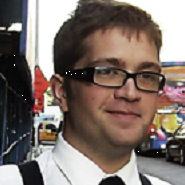
\includegraphics[width=150pt]{authors/scox.jpg}} &
	\cellcolor[rgb]{0.798,0.898,0.764}
	\vspace{3pt}
	\hspace*{2pt}
	\parbox{270pt}{
		\textcolor[rgb]{0.166,0.313,0.115}{\textbf{Sean Cox}}
		is an Analyst at RatPac-Dune Entertainment. He is an expert in mathematics of finance and econometrics. Previously he worked for The Blackstone Group as mathematician and analyst. In his spare time he pursues outdoor activities.
		\bigskip
		\par 
		\textcolor[rgb]{0.136,0.232,0.102}\Letter~~\href{mailto:sean.cox@ratpacent.com}{\color[rgb]{0.136,0.232,0.102}sean.cox@ratpacent.com}
	}
	\\
\end{tabular}



\end{document}
